\chapter{Potential Beam Use Proposal 2026--2027}
\label{chap:beam_use_proposal_extra}

In this Chapter we provide details on a potential additional two years of running in 2026--2027 that presents a further return on investment in sPHENIX and also the entire RHIC program.   We highlight if such a window of opportunity arises this would represent the last opportunity for data taking in heavy-ion mode in this energy regime in our lifetime. 

\section{Proposal Summary}

The sPHENIX proposal for such a potential window of opportunity is summarized in Table~\ref{tab:summary2627}.   The two years assume 28 cryo-weeks in each and with a sPHENIX uptime of 80\% with detector operations having reached a mature state.   Projected luminosities are documented by these years 2026 and 2027 by C-AD.  For completeness we detail in the cryo-weeks for the potential 2026 and 2027 runs at the end of this Chapter in Section~\ref{sec:cryo20262027}.

\begin{table}[h!]
\centering
\caption{The recorded luminosity (Rec. Lum.) and sampled luminosity (Samp. Lum.) values are for collisions with z-vertex $|z|<$ 10 cm.  \label{tab:summary2627}}
\bigskip
\centering
\begin{tabular}{ | c | c | c | c | c | c | c  | }
\hline
Year & Species & $\sqrt{s_{NN}}$ & Cryo  & Physics & Rec. Lum. & Samp. Lum. \\
     &         & [GeV]           & Weeks & Weeks   & $|z|<$10~cm & $|z|<$10~cm  \\ \hline \hline
     {2026} & $p^{\uparrow}p^{\uparrow}$   & 200 & 28 & 15.5      & 1.0 \pb [10 kHz]   & 80 \pb \\ 
      & & & & & 80~\pb [100\%-$str$] & \\ \hline
       --  & O+O    & 200 & -- & 2        & 18~\nb & 37~\nb  \\ 
       & & & & & 37~\nb [100\%-$str$] & \\ \hline
 --  & Ar+Ar   & 200 & -- & 2      & 6~\nb  & 12~\nb  \\ 
        & & & & & 12~\nb [100\%-$str$] & \\ \hline \hline
{{2027}} & \auau   & 200 & 28 & 24.5 & 30 \nb [100\%-$str$/DeMux]   & 30 \nb \\ \hline
\end{tabular}

\end{table}

We highlight that key upgrades at very modest cost are a major factor increasing the physics impact of these additional years of running.   Demultiplexing the calorimeter readout increases the Level-1 trigger accept rate to 30 kHz, doubling the rate of calorimeter data events.    Increasing the tracking detectors streaming readout to 100\% results in an order of magnitude more data than in the 2024-2025 data taking.    These upgrade options are detailed in Chapter~\ref{chap:readout}.

%\section{Physics Projections}
%We detail the potential physics gain from the 2026 and 2027 running in the following two subsections, focusing %first on the additional \auau and \pp running and then on the novel system O+O and Ar+Ar running.

\newpage
\section{\auau and \pp Physics Reach}

First, we start with the \auau increased physics reach.    In Table~\ref{tab:auau2027} we compare directly the \auau recorded and sampled luminosities from the three runs in 2023, 2025, and the potential opportunity in 2027.   The upgrades enable a doubling of the \auau data set to 30 nb$^{-1}$ or equivalently 200 billion \auau events.    These events are a permanent archive of \auau data to be mined for any future analysis once the RHIC machine is not longer running heavy ions.    There are no trigger biases or selections that would preclude any analysis within the acceptance and performance parameters of sPHENIX.

\begin{table}[h]
\centering
\caption{Summary of Au+Au at 200 GeV option sPHENIX Beam Use Proposal.
The recorded luminosity (Rec. Lum.) and first sampled luminosity (Samp. Lum.) values are for collisions with z-vertex $|z|<$ 10 cm.  The final column shows the sampled luminosity for all z-vertex values, relevant for calorimeter only measurements.\label{tab:auau2027}}
\bigskip
\centering
\begin{tabular}{ | c | c | c | c | c | c | c  | }
\hline
Year & Species & $\sqrt{s_{NN}}$ & Cyro  & Physics & Rec. Lum. & Samp. Lum. \\
     &         & [GeV]           & Weeks & Weeks   & $|z|<$10~cm & $|z|<$10~cm  \\ \hline \hline

2023 & \auau   & 200 & 24 (28) & 9 (13) & 3.7 (5.7) \nb   & 4.5 (6.9) \nb  \\ \hline
2025 & \auau   & 200 & 24 (28) & 20.5 (24.5) & 13 (15) \nb   & 21 (25) \nb  \\ \hline
{\bf{2027}} & \auau   & 200 & 28 & 24.5 & 30 \nb [100\%-$str$/DeMux]   & 31 \nb \\ \hline
\end{tabular}
\end{table}

The impact on the \pp data set is even more substantial.   The comparison of running \pp in 2024 and 2026 is shown in Table~\ref{tab:2026pp}.   The striking gain is in the 130~\pb recorded with the tracking detectors via 100\%-$str$ mode, more than a factor of ten over the previous data set.    There are many measurements, particularly in the heavy-flavor and transverse spin (cold QCD) arena where selecting physics triggers are not available and thus the \pp measurements are the statistical limitation in nuclear modification factors.    This enormous data set both for calorimetric jets with 130~\pb additional sampled and for all channels available via the tracking detectors with 130~\pb recorded again represents an immediate opportunity to advance our precision physics knowledge and a permanent archive of data from RHIC.

\begin{table}[h]
\centering
\caption{The recorded luminosity (Rec. Lum.) and sampled luminosity (Samp. Lum.) values are for collisions with z-vertex $|z|<$ 10 cm.  \label{tab:2026pp}}
\bigskip
\centering
\begin{tabular}{ | c | c | c | c | c | c | c  | }
\hline
Year & Species & $\sqrt{s_{NN}}$ & Cyro  & Physics & Rec. Lum. & Samp. Lum. \\
     &         & [GeV]           & Weeks & Weeks   & $|z|<$10~cm & $|z|<$10~cm  \\ \hline \hline
2024 & $p^{\uparrow}p^{\uparrow}$     & 200 & 24 (28) & 12 (16) & 0.3 (0.4) \pb [5 kHz] & 73 (101) \pb  \\
     &                                &     &  & &  7.3 (10.1) \pb [10\%-$str$]&   \\ \hline
     {\bf 2026} & $p^{\uparrow}p^{\uparrow}$   & 200 & 28 & 15.5      & 1.0 \pb [10 kHz]   & 130 \pb \\ 
      & & & & & 130~\pb [100\%-$str$] & \\ \hline
\end{tabular}
\end{table}

The substantial gain in statistics translates into super-precise measurements of basic observables and the enabling of highly differential observables.    Here we show a subset of example projection plots.   Figure~\ref{fig:RAA_jet_extrayears} (left) shows the improvement in statistical precision for direct photon, jet, and charged hadron nuclear modification factor R$_{AA}$ as a function of $p_T$ in 0-10\% central \auau collisions.    The improved statistics, particularly at high-$p_{T}$ where underlying event backgrounds are low, enable a precision decomposition of these jet events.   Figure~\ref{fig:RAA_jet_extrayears} (right) shows the statistical precision for the ``golden-channel'' photon + jet distribution.    The precision is sufficient that one can then further dissect these events and look for medium response opposite the photon in selections of $x_{J\gamma}$.   Another example of a statistics hungry measurement is the azimuthal anisotropy of high $p_T$ probes.    Figure~\ref{fig:jet_dphi_proj} shows the statistical uncertainties for jets with $p_{T} > 40$~GeV as a function of angle relative to the second-order reaction plane.    The precision measurements with Year 4-5 (2026 - 2027) data included will enable a key constraint on jet quenching calculations embedded in realistic hydrodynamic expanding background.

\begin{figure}
    \centering
    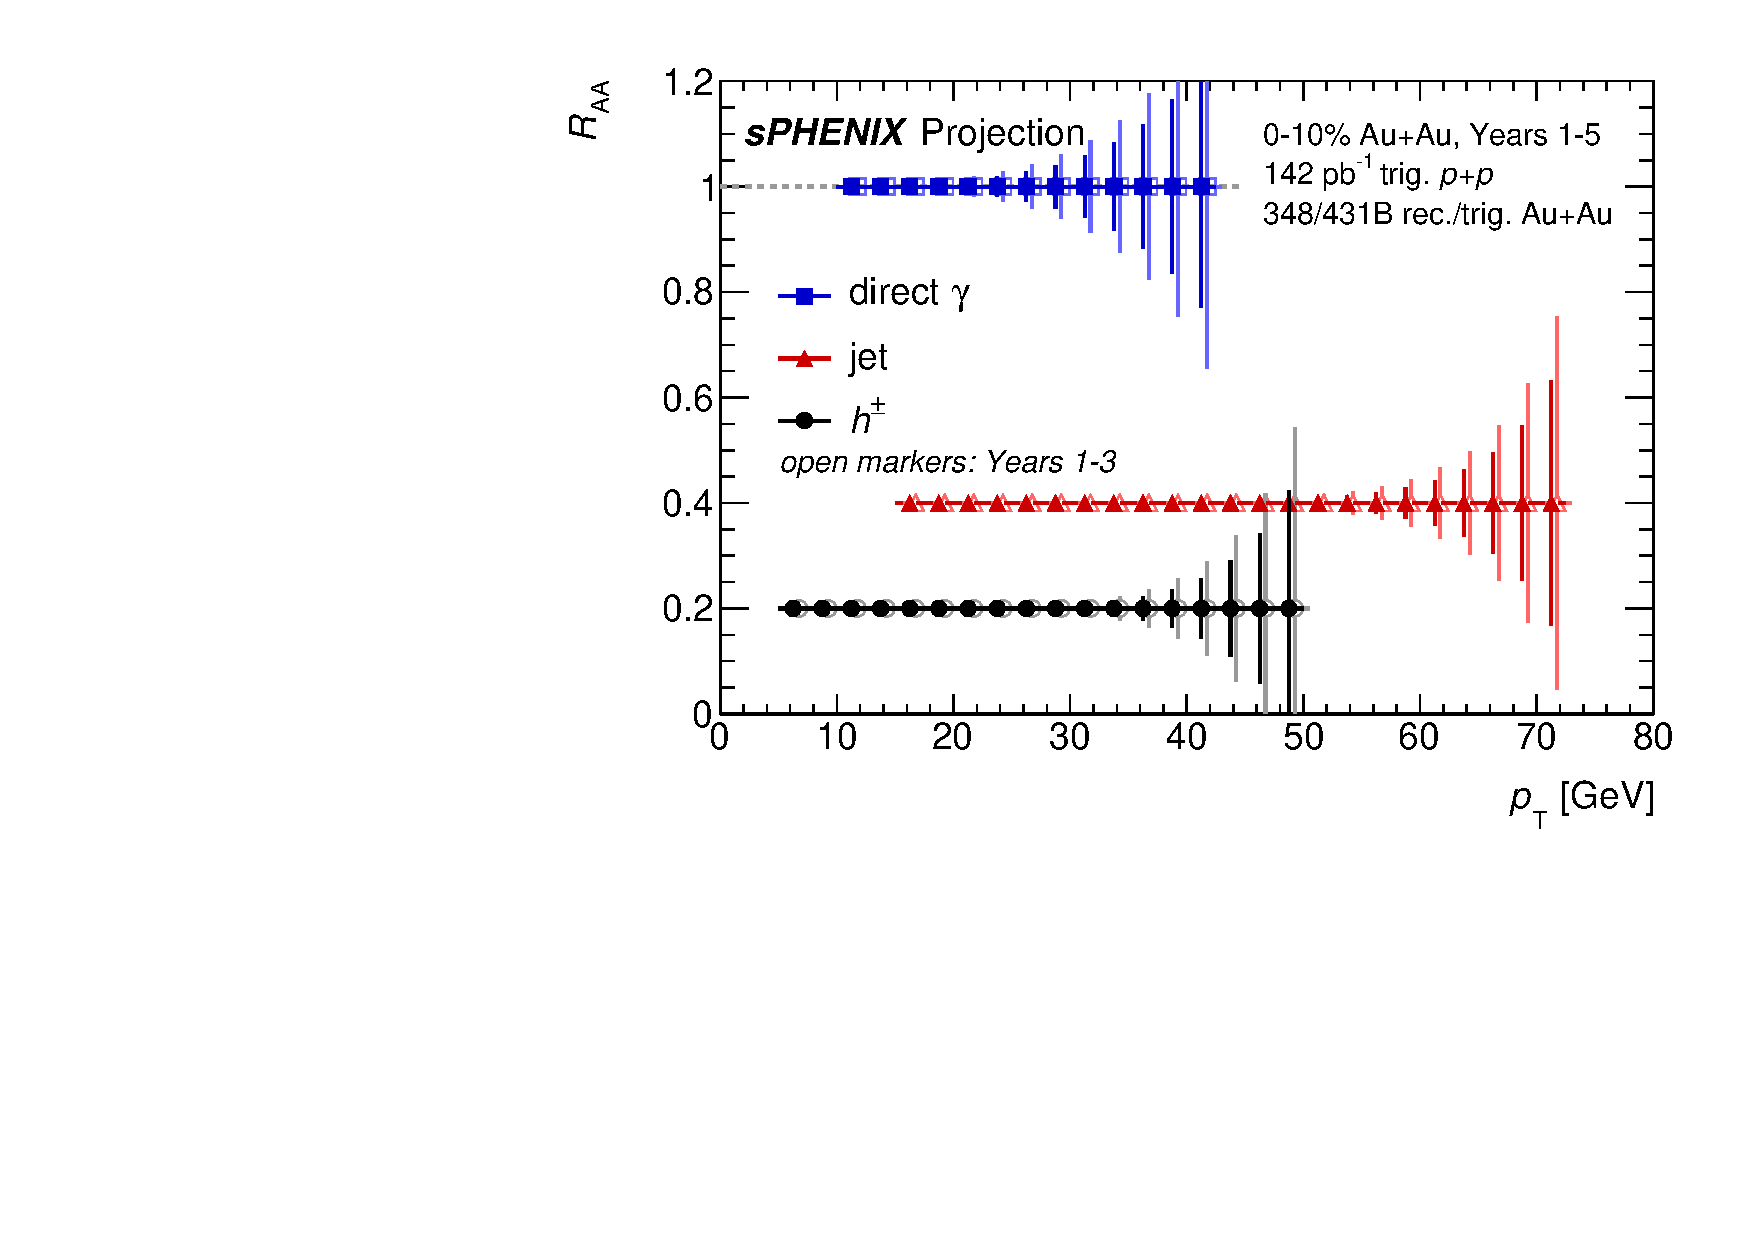
\includegraphics[width=0.48\linewidth]{figs/RAA_jet_2}
    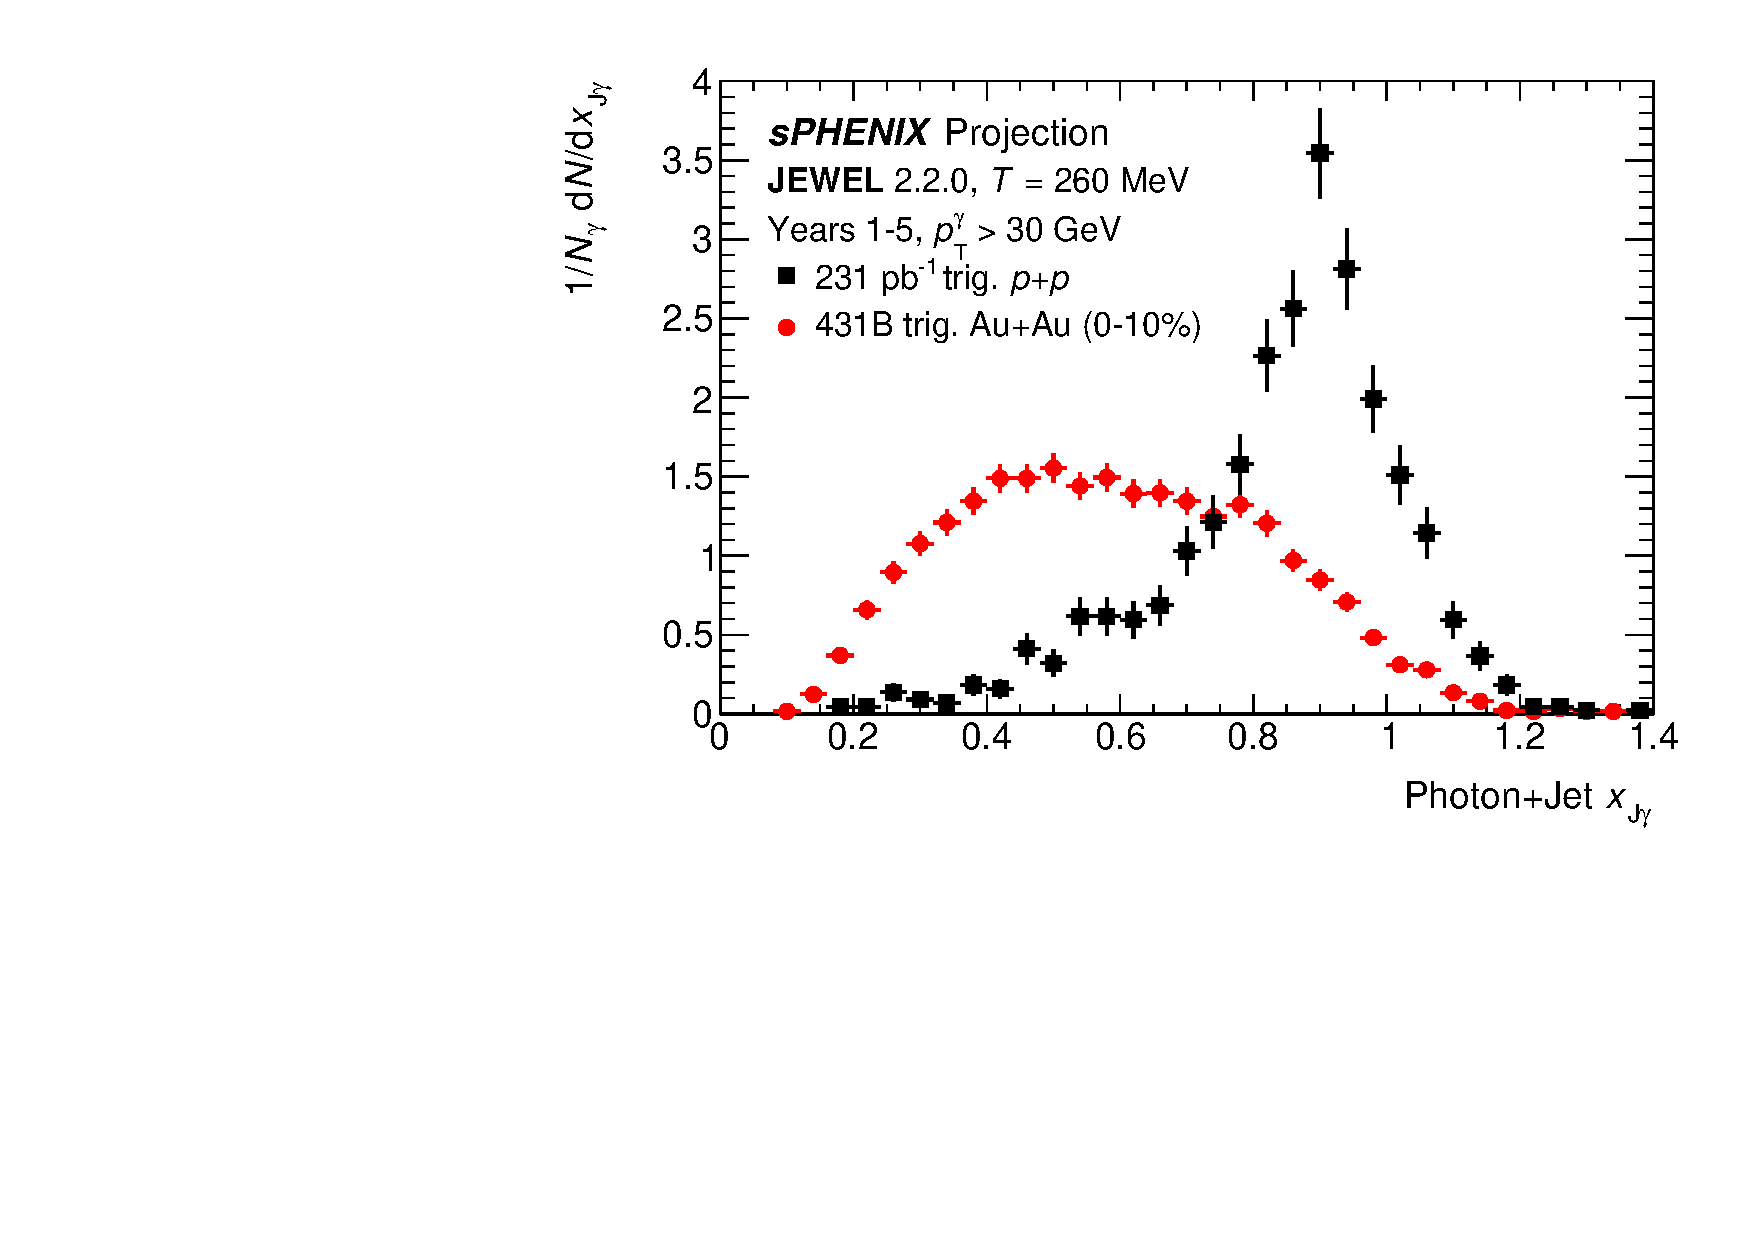
\includegraphics[width=0.48\linewidth]{figs/xJg_2}
    \caption{(left) Nuclear modification factor R$_{AA}$ in 0-10\% central \auau collisions for direct photons, jets, and charged hadrons as a function of $p_T$.   Shown are the statistical uncertainties from Year 1-3 (2023-2025) running compared with including the additional Year 4-5 (2026-2027) running.   (right). Statistical precision for $x_{J\gamma}$ in photon + jet events from additional Year 4-5 (2026-2027) running.}
    \label{fig:RAA_jet_extrayears}
\end{figure}

\begin{figure}[h]
\centering
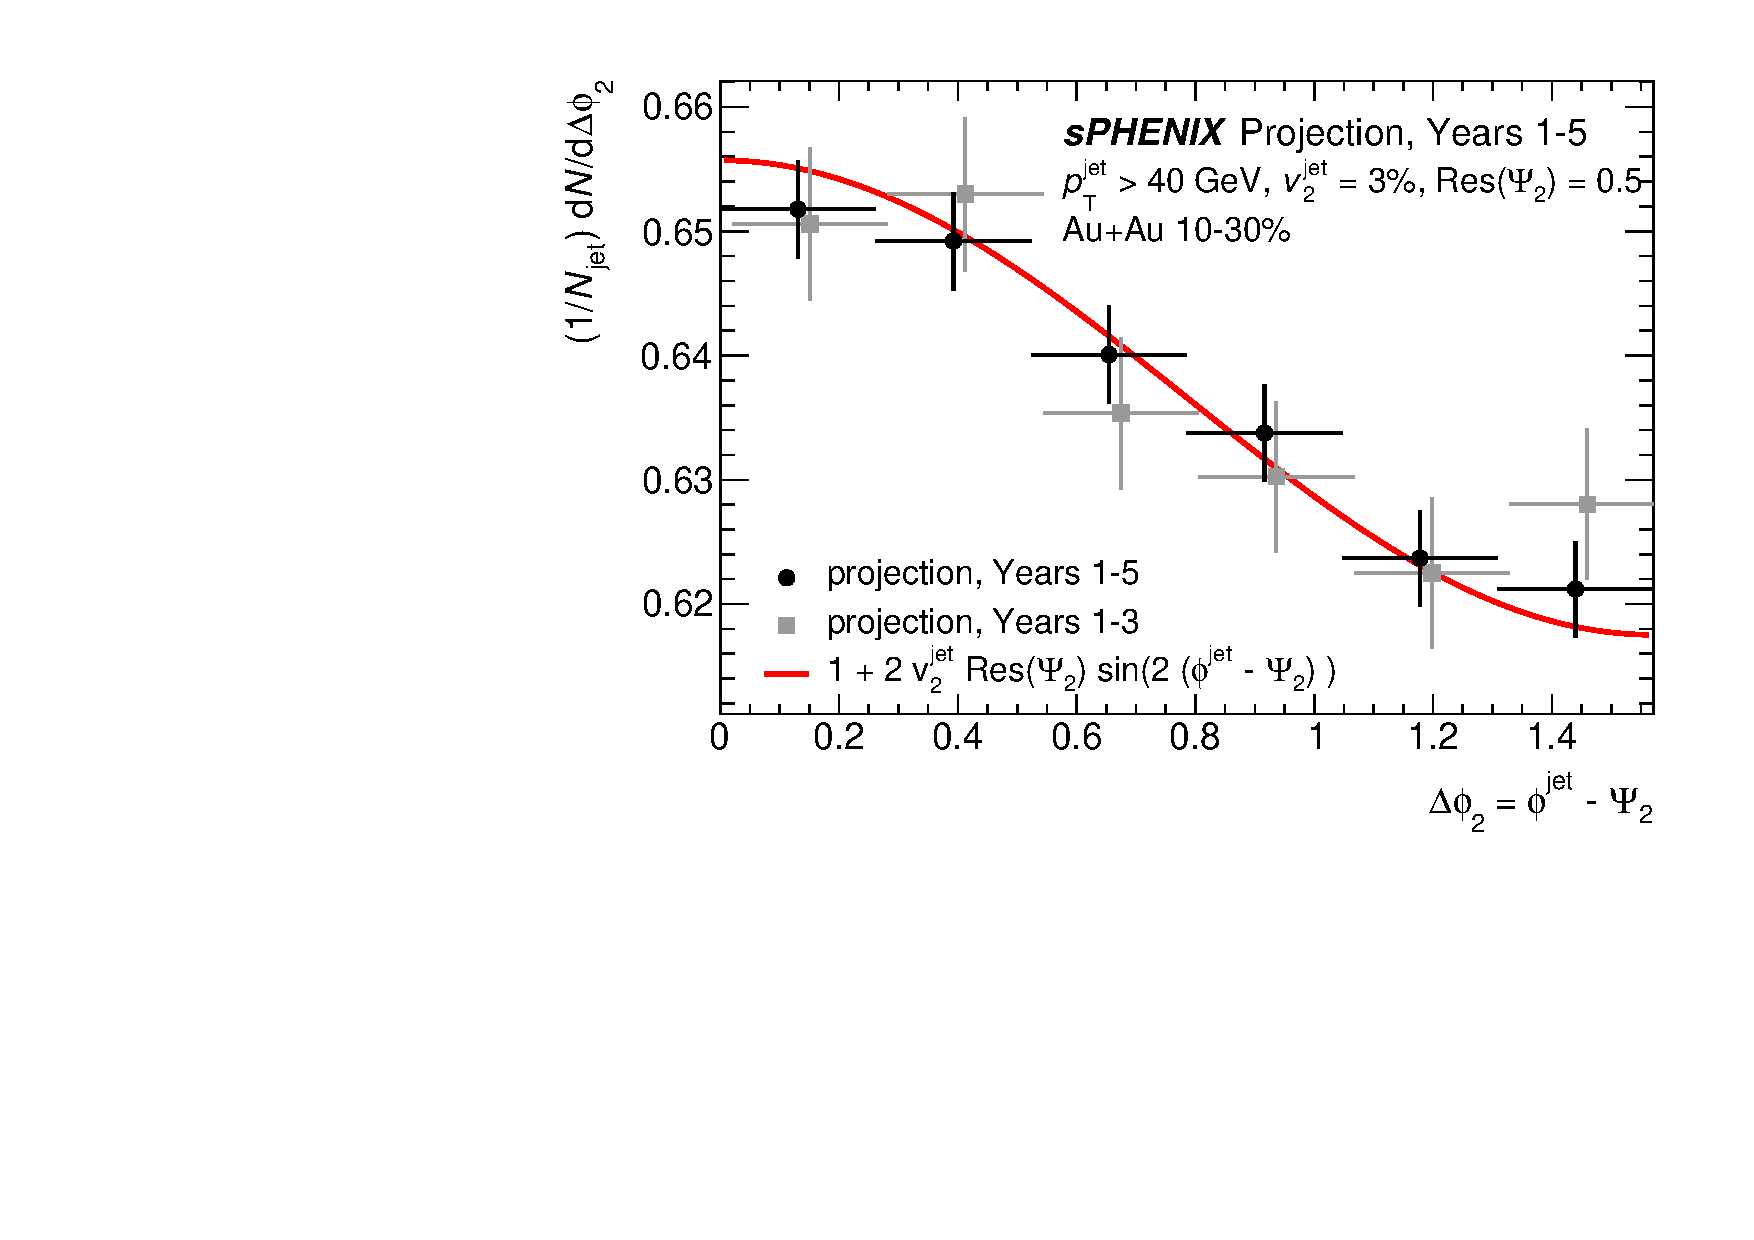
\includegraphics[width=0.48\textwidth]{figs/jet_dphi_2}
\caption{Statistical projections for the jet yield as a function of the azimuthal distance from the event plane in 10--30\% Au+Au events.}
\label{fig:jet_dphi_proj}
\end{figure}

The Upsilon measurement is another case where additional statistical precision enables more differential observations.   Figure~\ref{fig:RAA_upsilon_extrayears} shows the increased statistical accuracy for the different states with the added Year 4-5 (2026-2027) data.     The improved statistics at lower $p_T$ will allow an examination of the properties of these events, for example azimuthal aniosotropies and other correlations measurements.

\begin{figure}
    \centering
    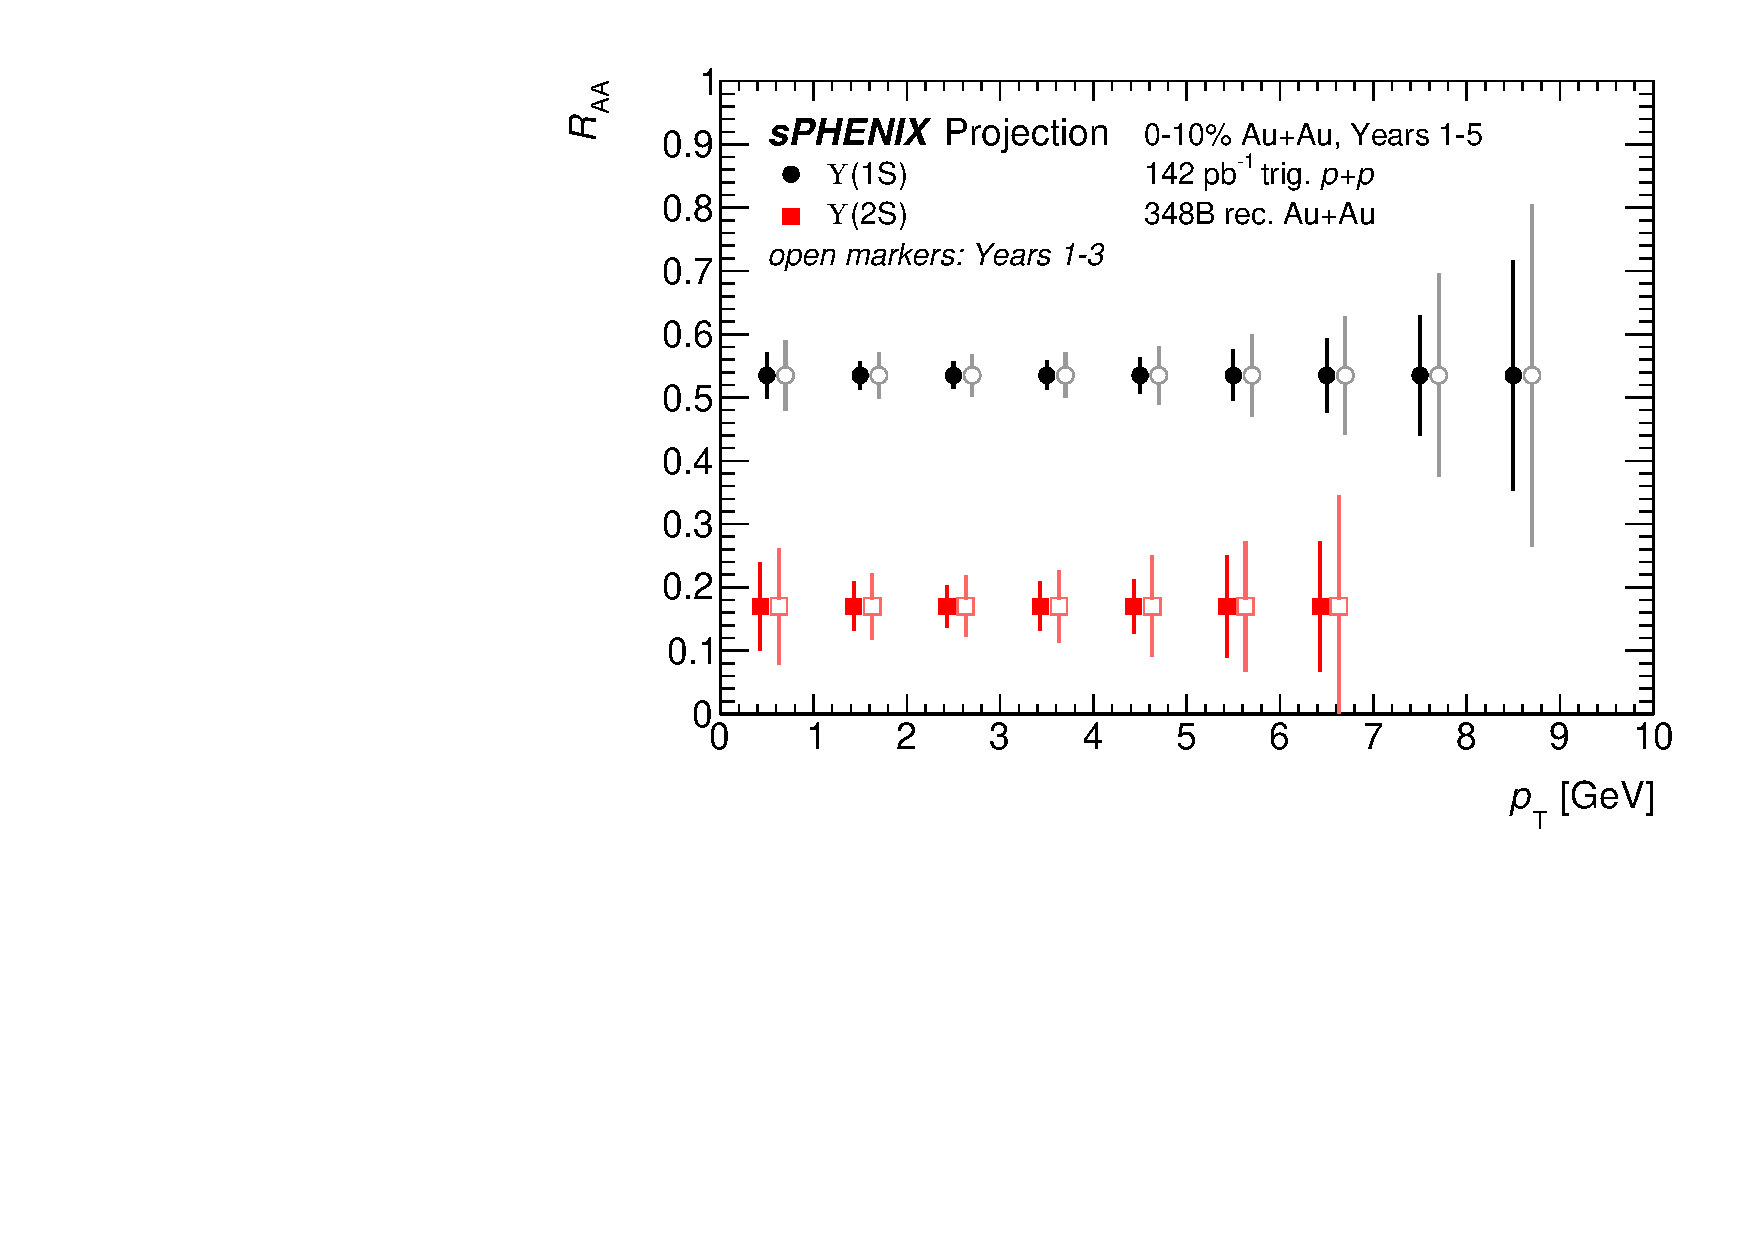
\includegraphics[width=0.50\linewidth]{figs/upsilon_RAA_2}
    \caption{sPHENIX projected statistical uncertainties,  including from background subtraction contributions, for the Upsilon nuclear modification factors in the proposed three-year (2023–2025) run plan and then compared with the improved precision adding projected data from 2026-2027.}
    \label{fig:RAA_upsilon_extrayears}
\end{figure}

The statistical gain from the 2026-2027 data would be beneficial for rare heavy-flavor observables, in particular for exclusive decay channels, HF flow and asymmetries. As shown in Figure~\ref{fig:v1-D0}, a clean separation of the the $v_1$ for $D^0$ and $\bar{D^0}$ is expected summing five year Au+Au data, which would provide quantitative access to the initial magnetic field in the HI collisions. With 100\% streaming DAQ, the $D^0$ statistics and uncertainty for the $D^0$ $A_N$ are dramatically improved in the polarized \pp collisions as shown in Figure~\ref{fig:AN-D0}, which provide a strong constraint on the tri-gluon correlations in the proton. 
The collaboration is also studying the viability of full reconstruction of exclusive decay channels such as $B_s$ meson that would provide new information on the strange enhancement and hadronization with the tagging of heavy bottom quark.  
 
\begin{figure}[h]
\begin{center}
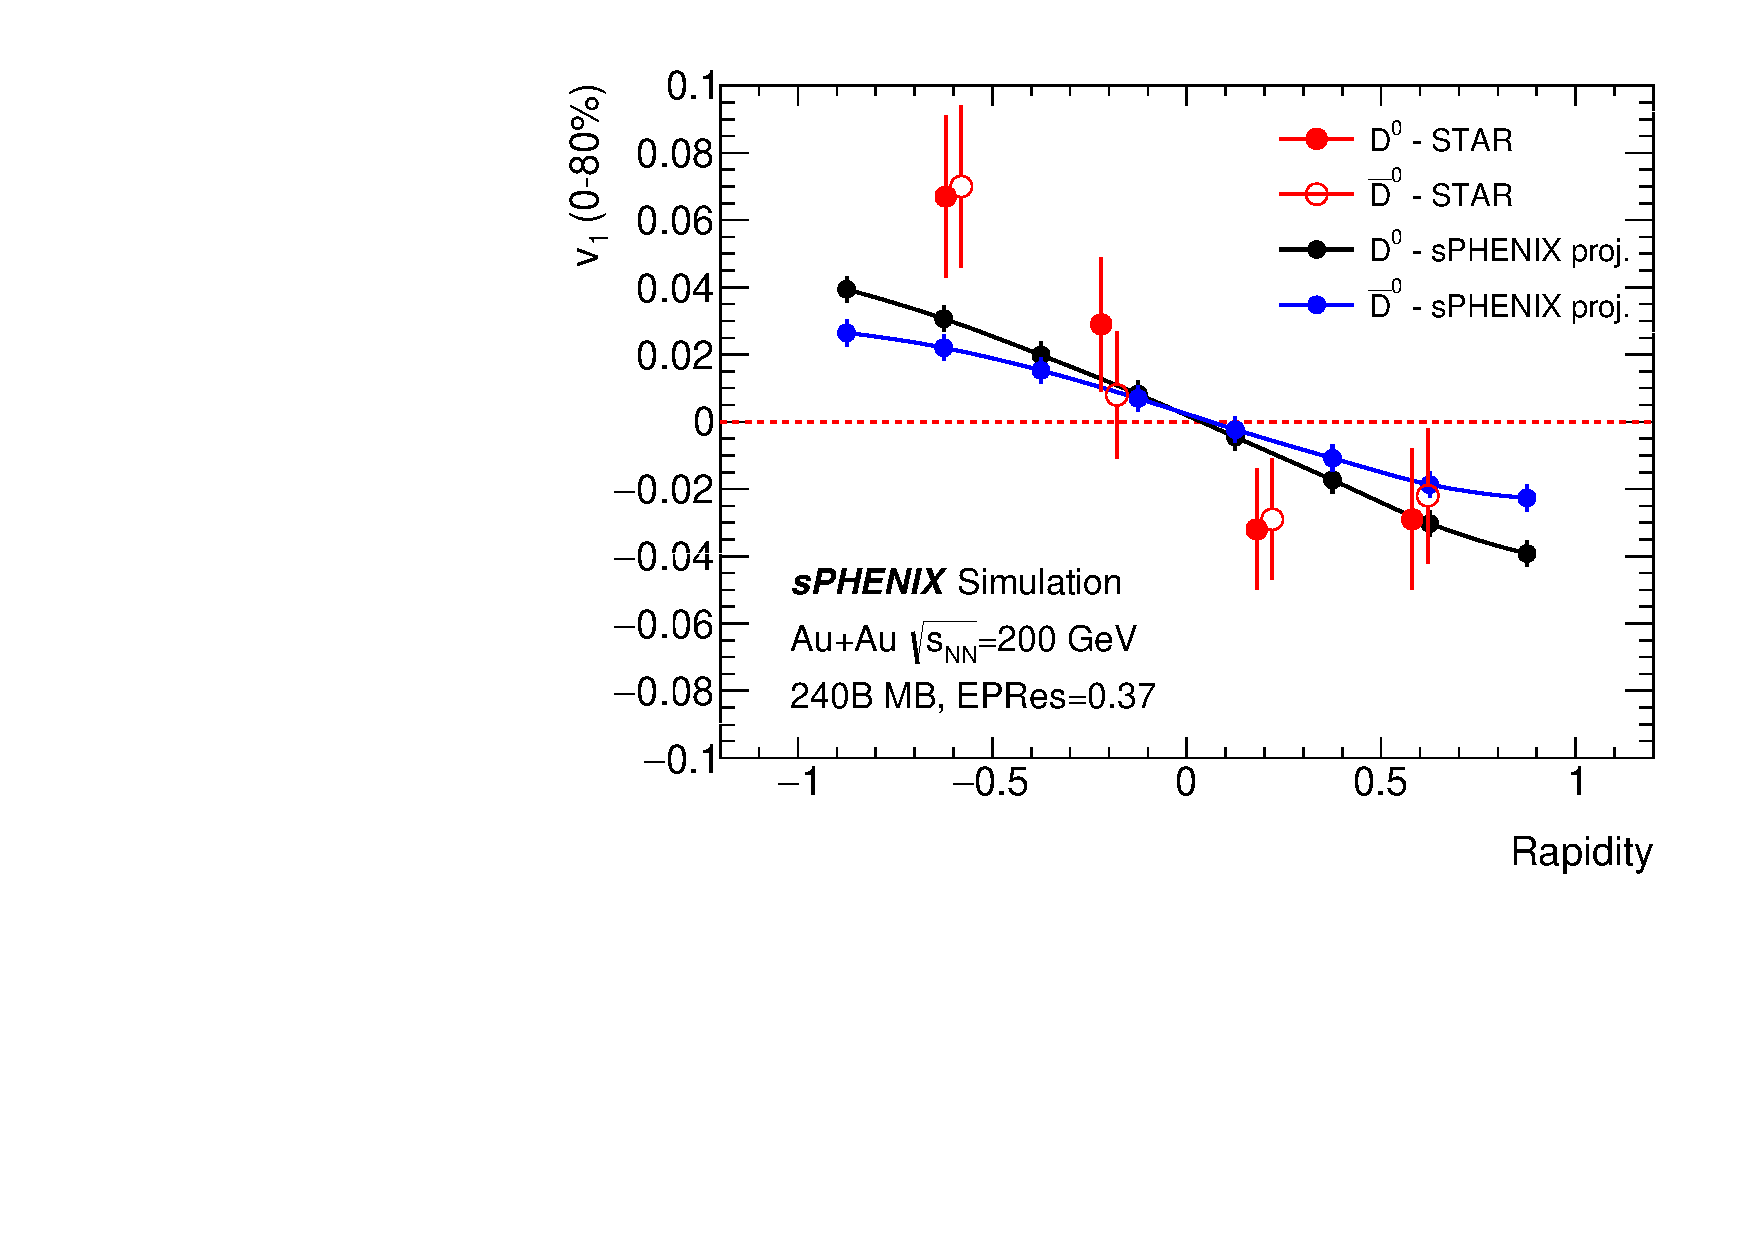
\includegraphics[width=.49\linewidth]{figs/v1_proj_240B_1.pdf}
% 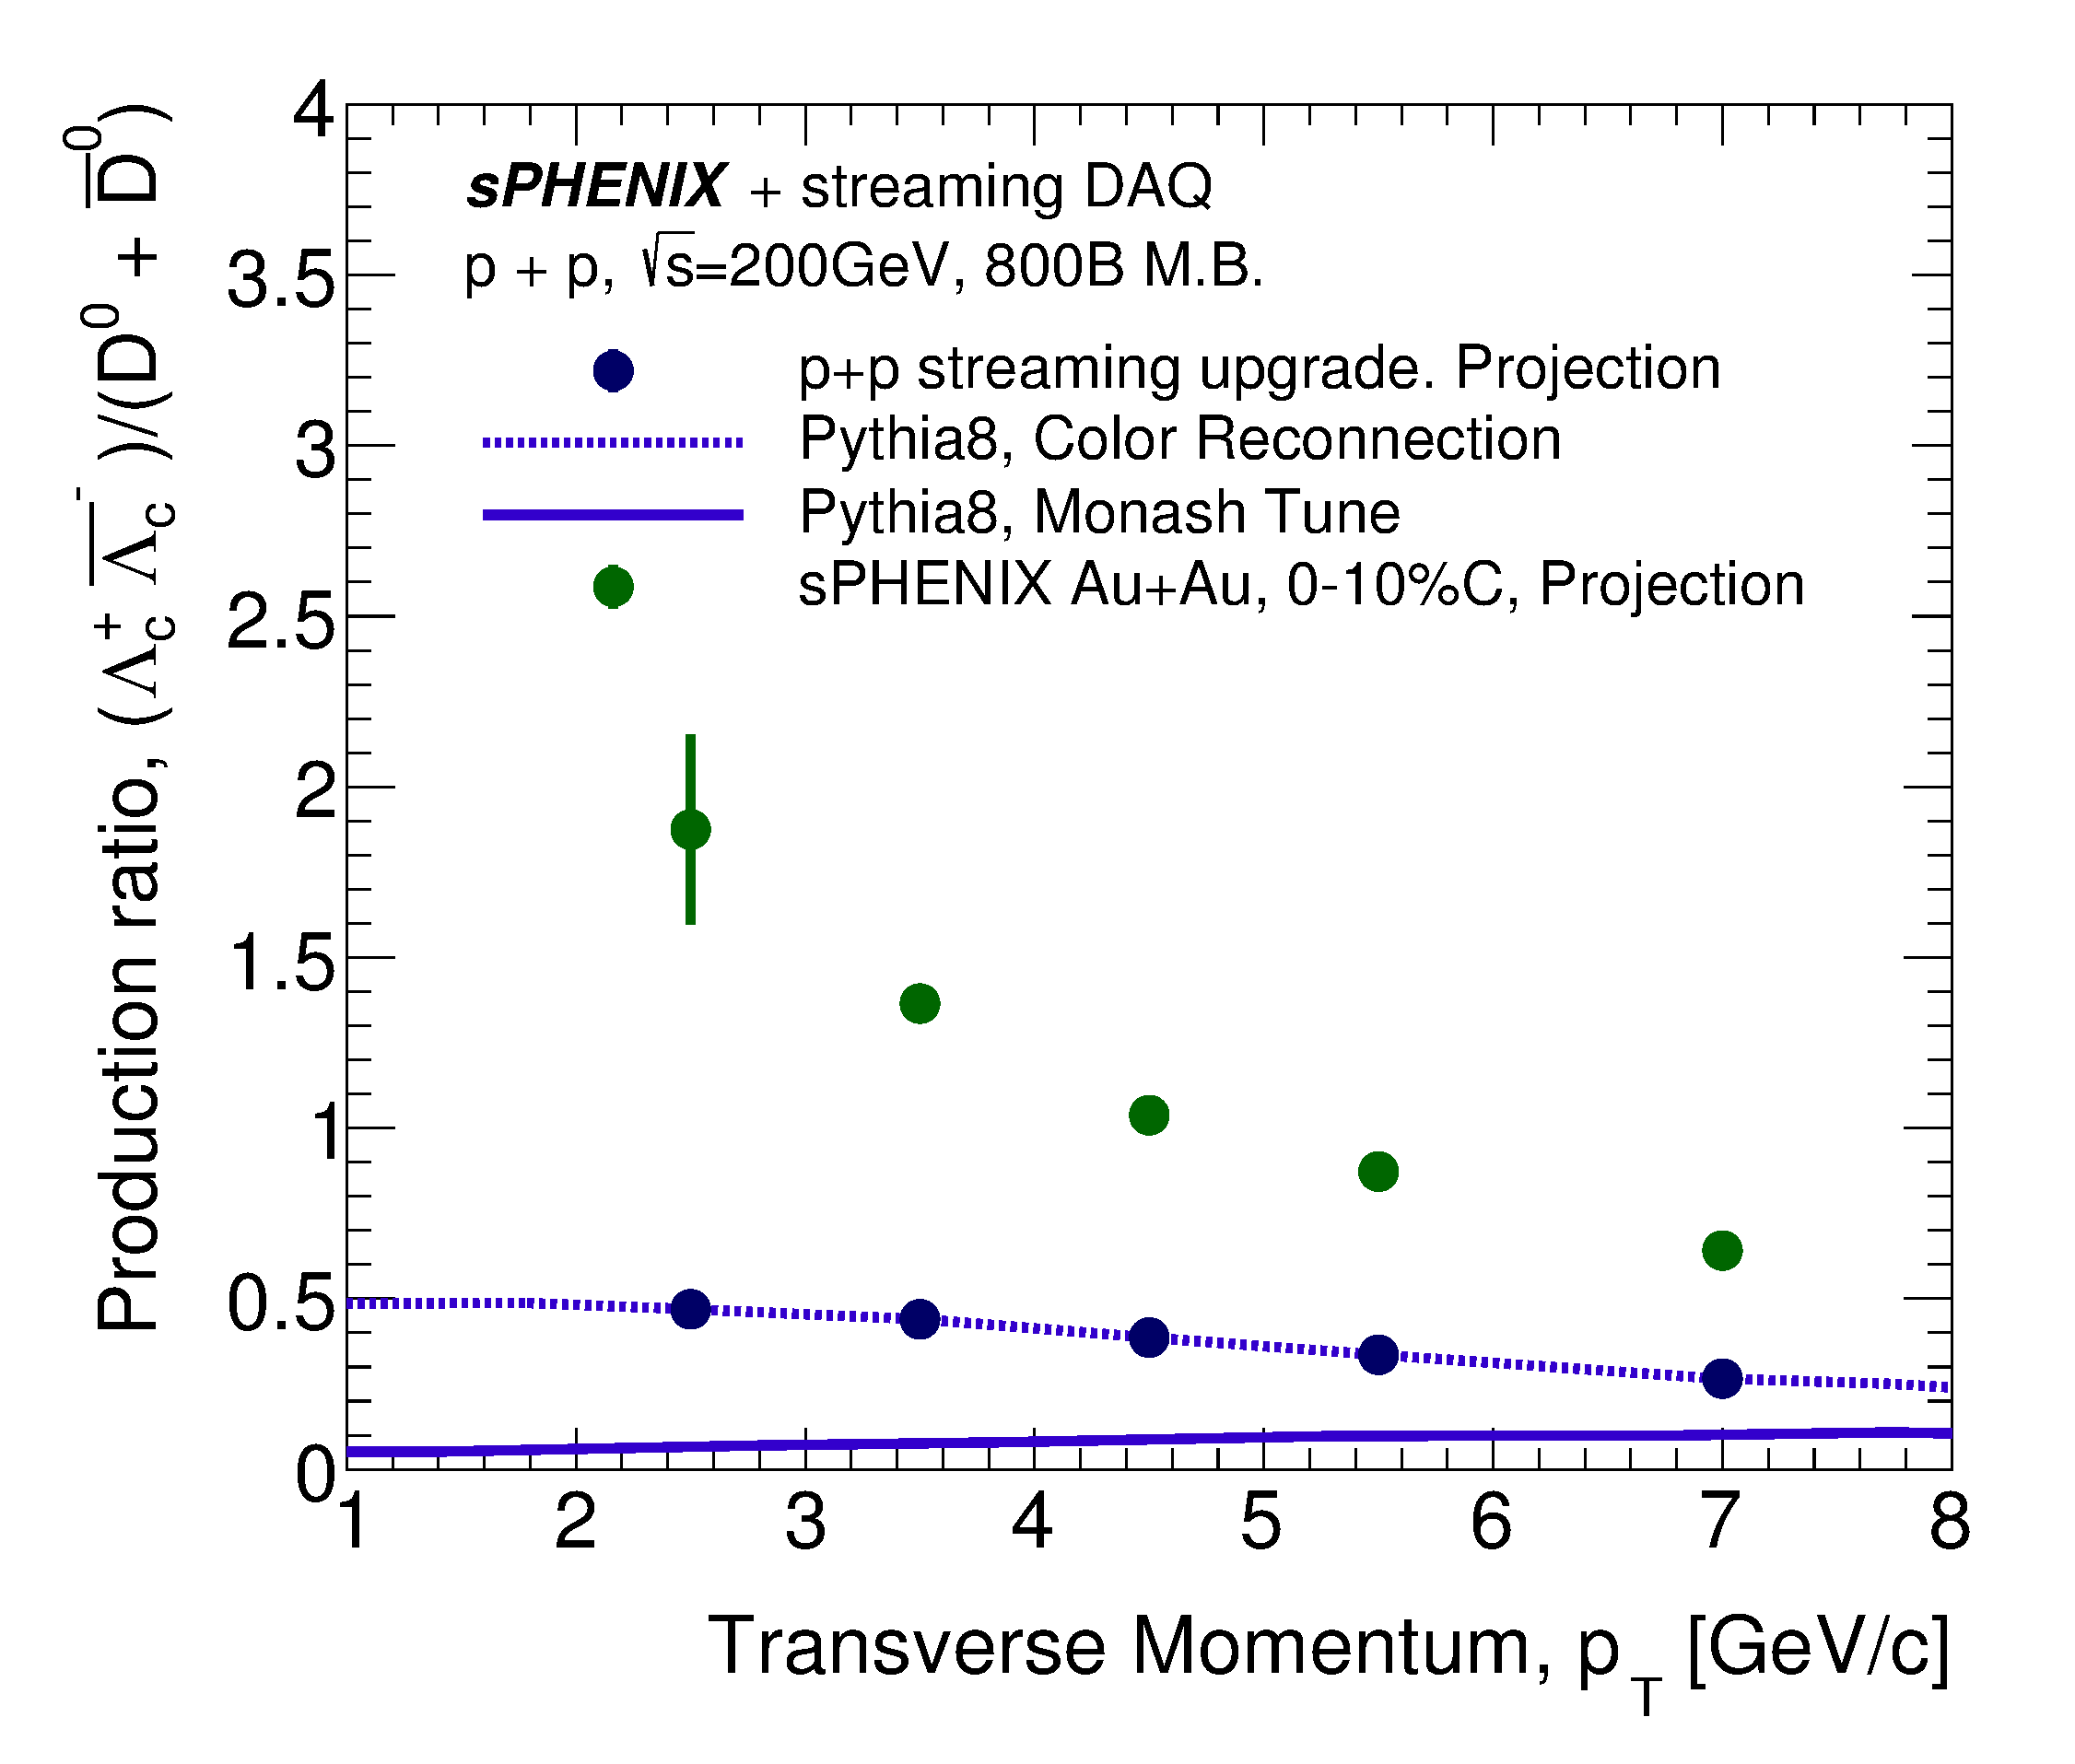
\includegraphics[width=.49\linewidth]{figs/RAA_DB_theory_root_LcD0Ratio.pdf}
\caption{ {\textcolor{red}{[plot to be updated with latest lumi]}}[Possible plot where  5-yr HF statistics is critical]Direct flow of $D^0$ meson.}
\label{fig:v1-D0}
\end{center}
\end{figure}
 


%\begin{figure}[htbp!]
\begin{figure}[h]
\begin{center}
% 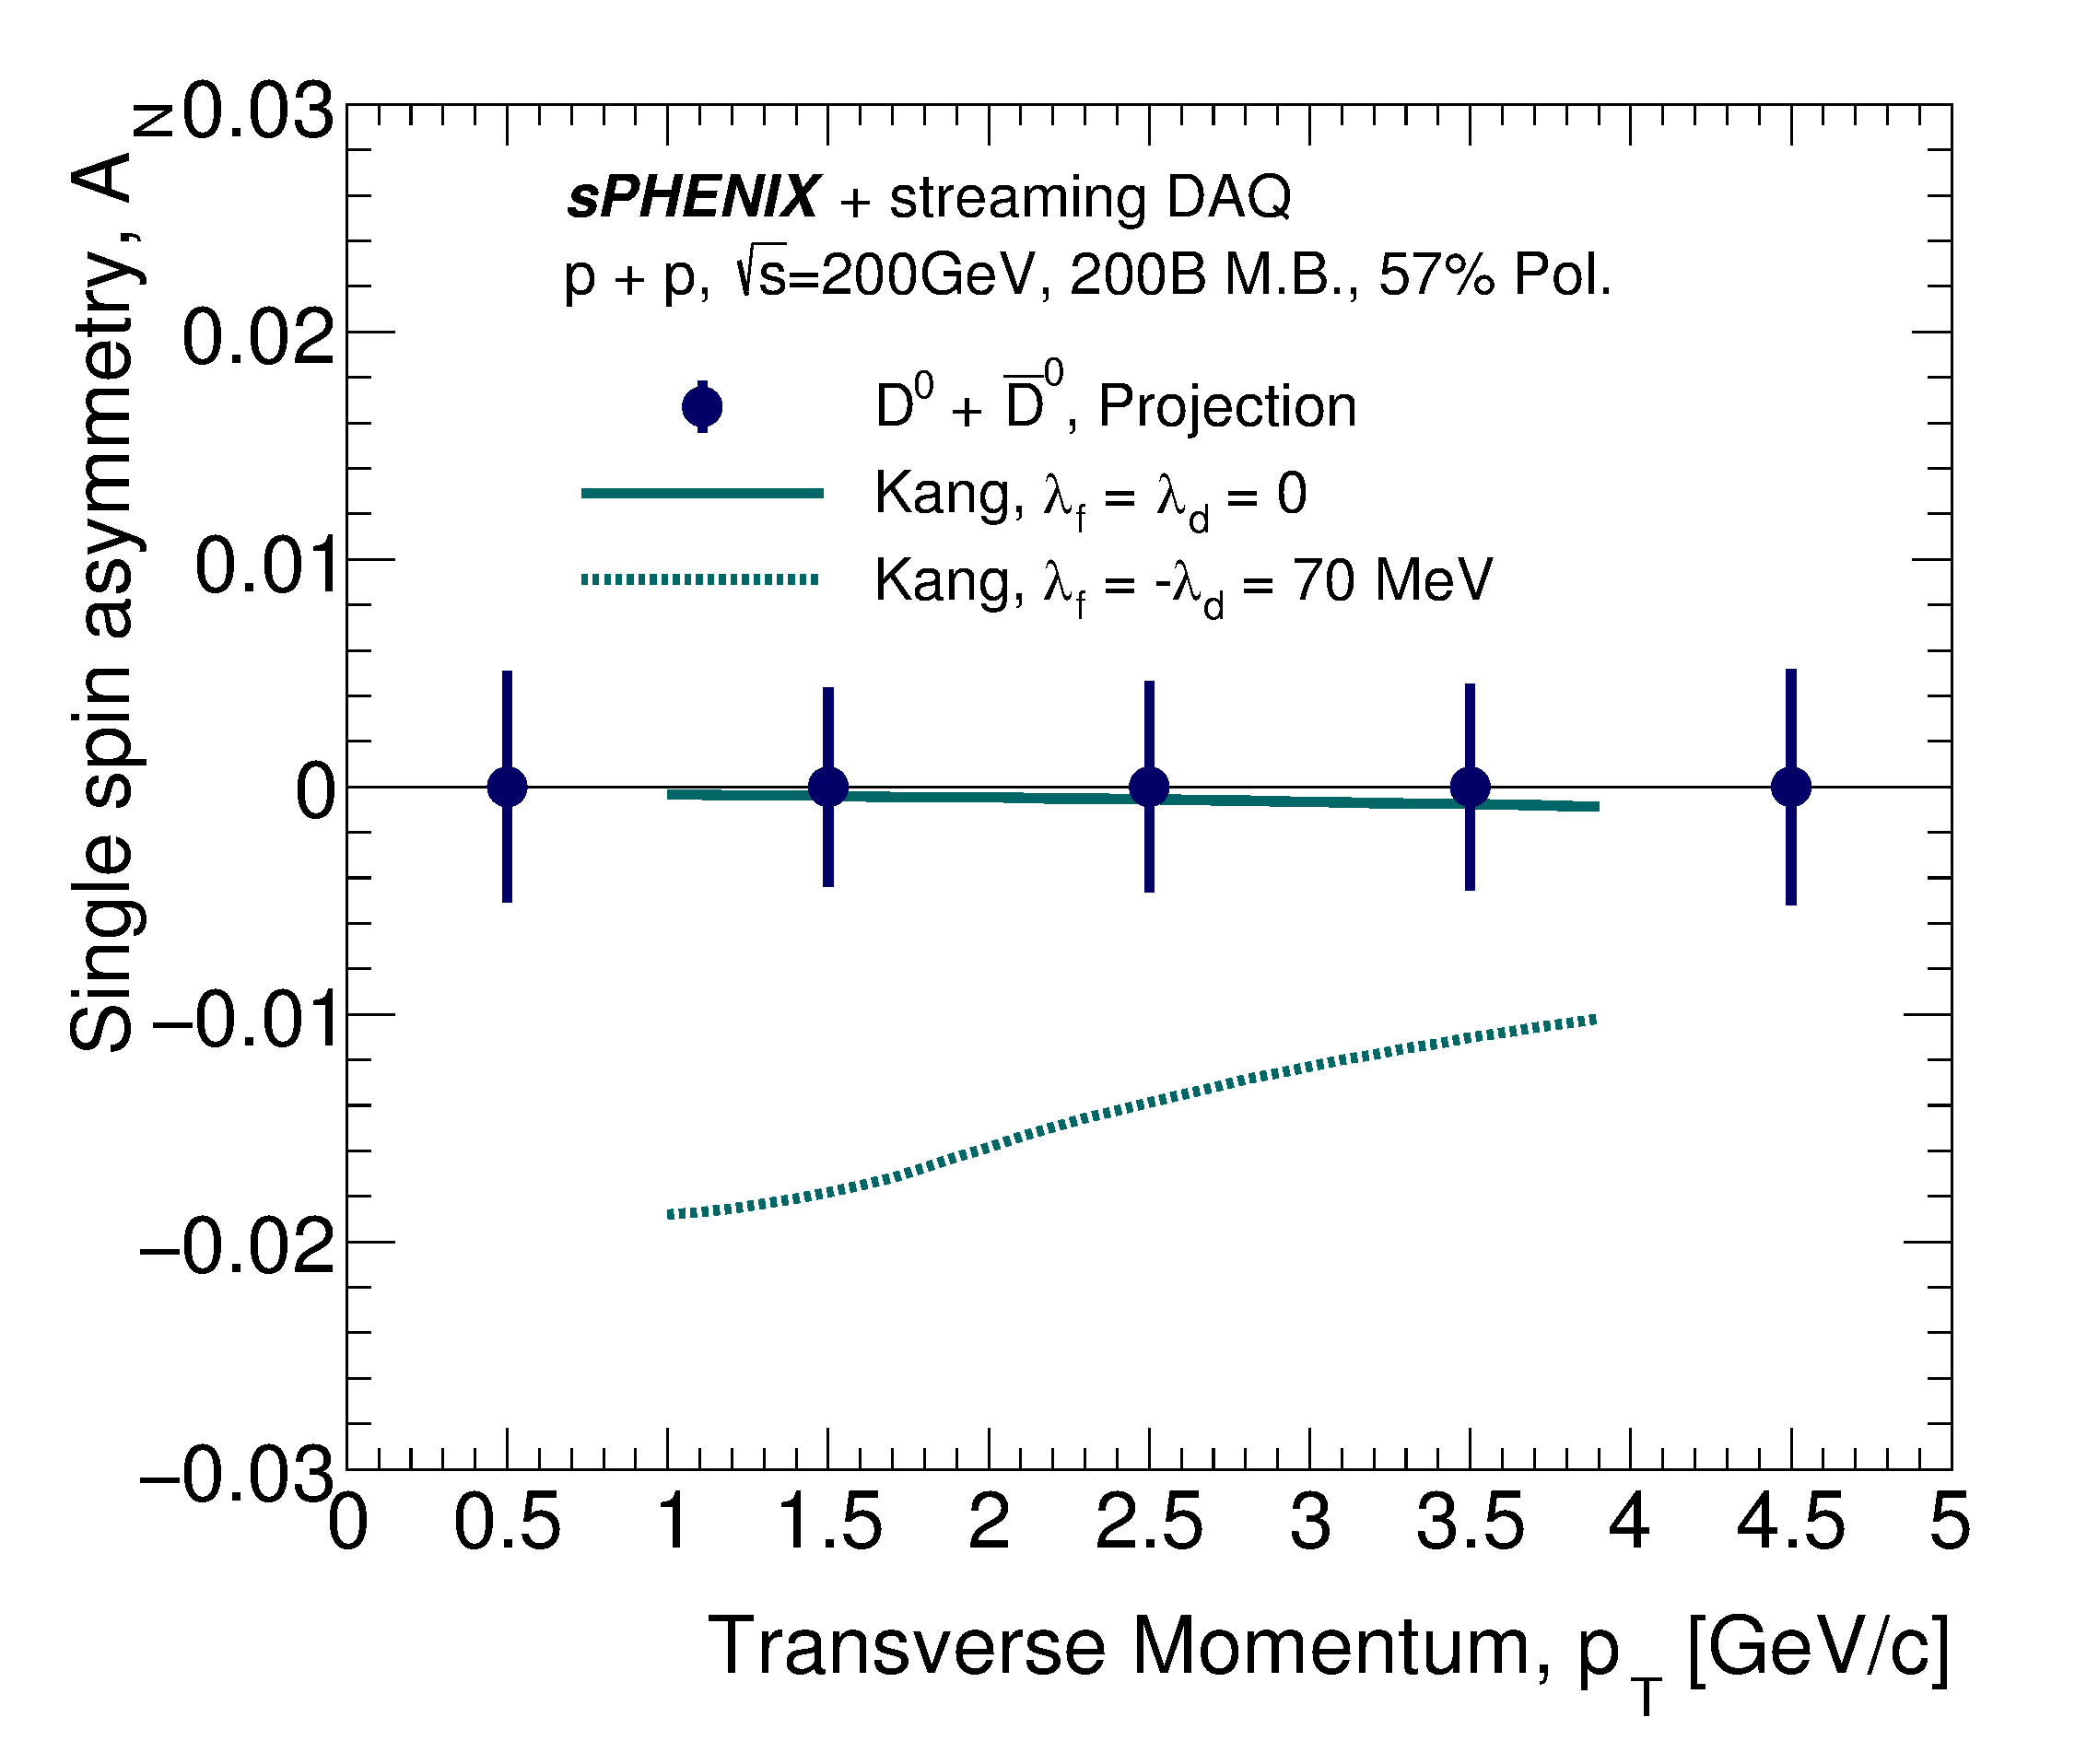
\includegraphics[width=.49\linewidth]{figs/RAA_DB_theory_root_AN_D0D0bar_pp200B.pdf}
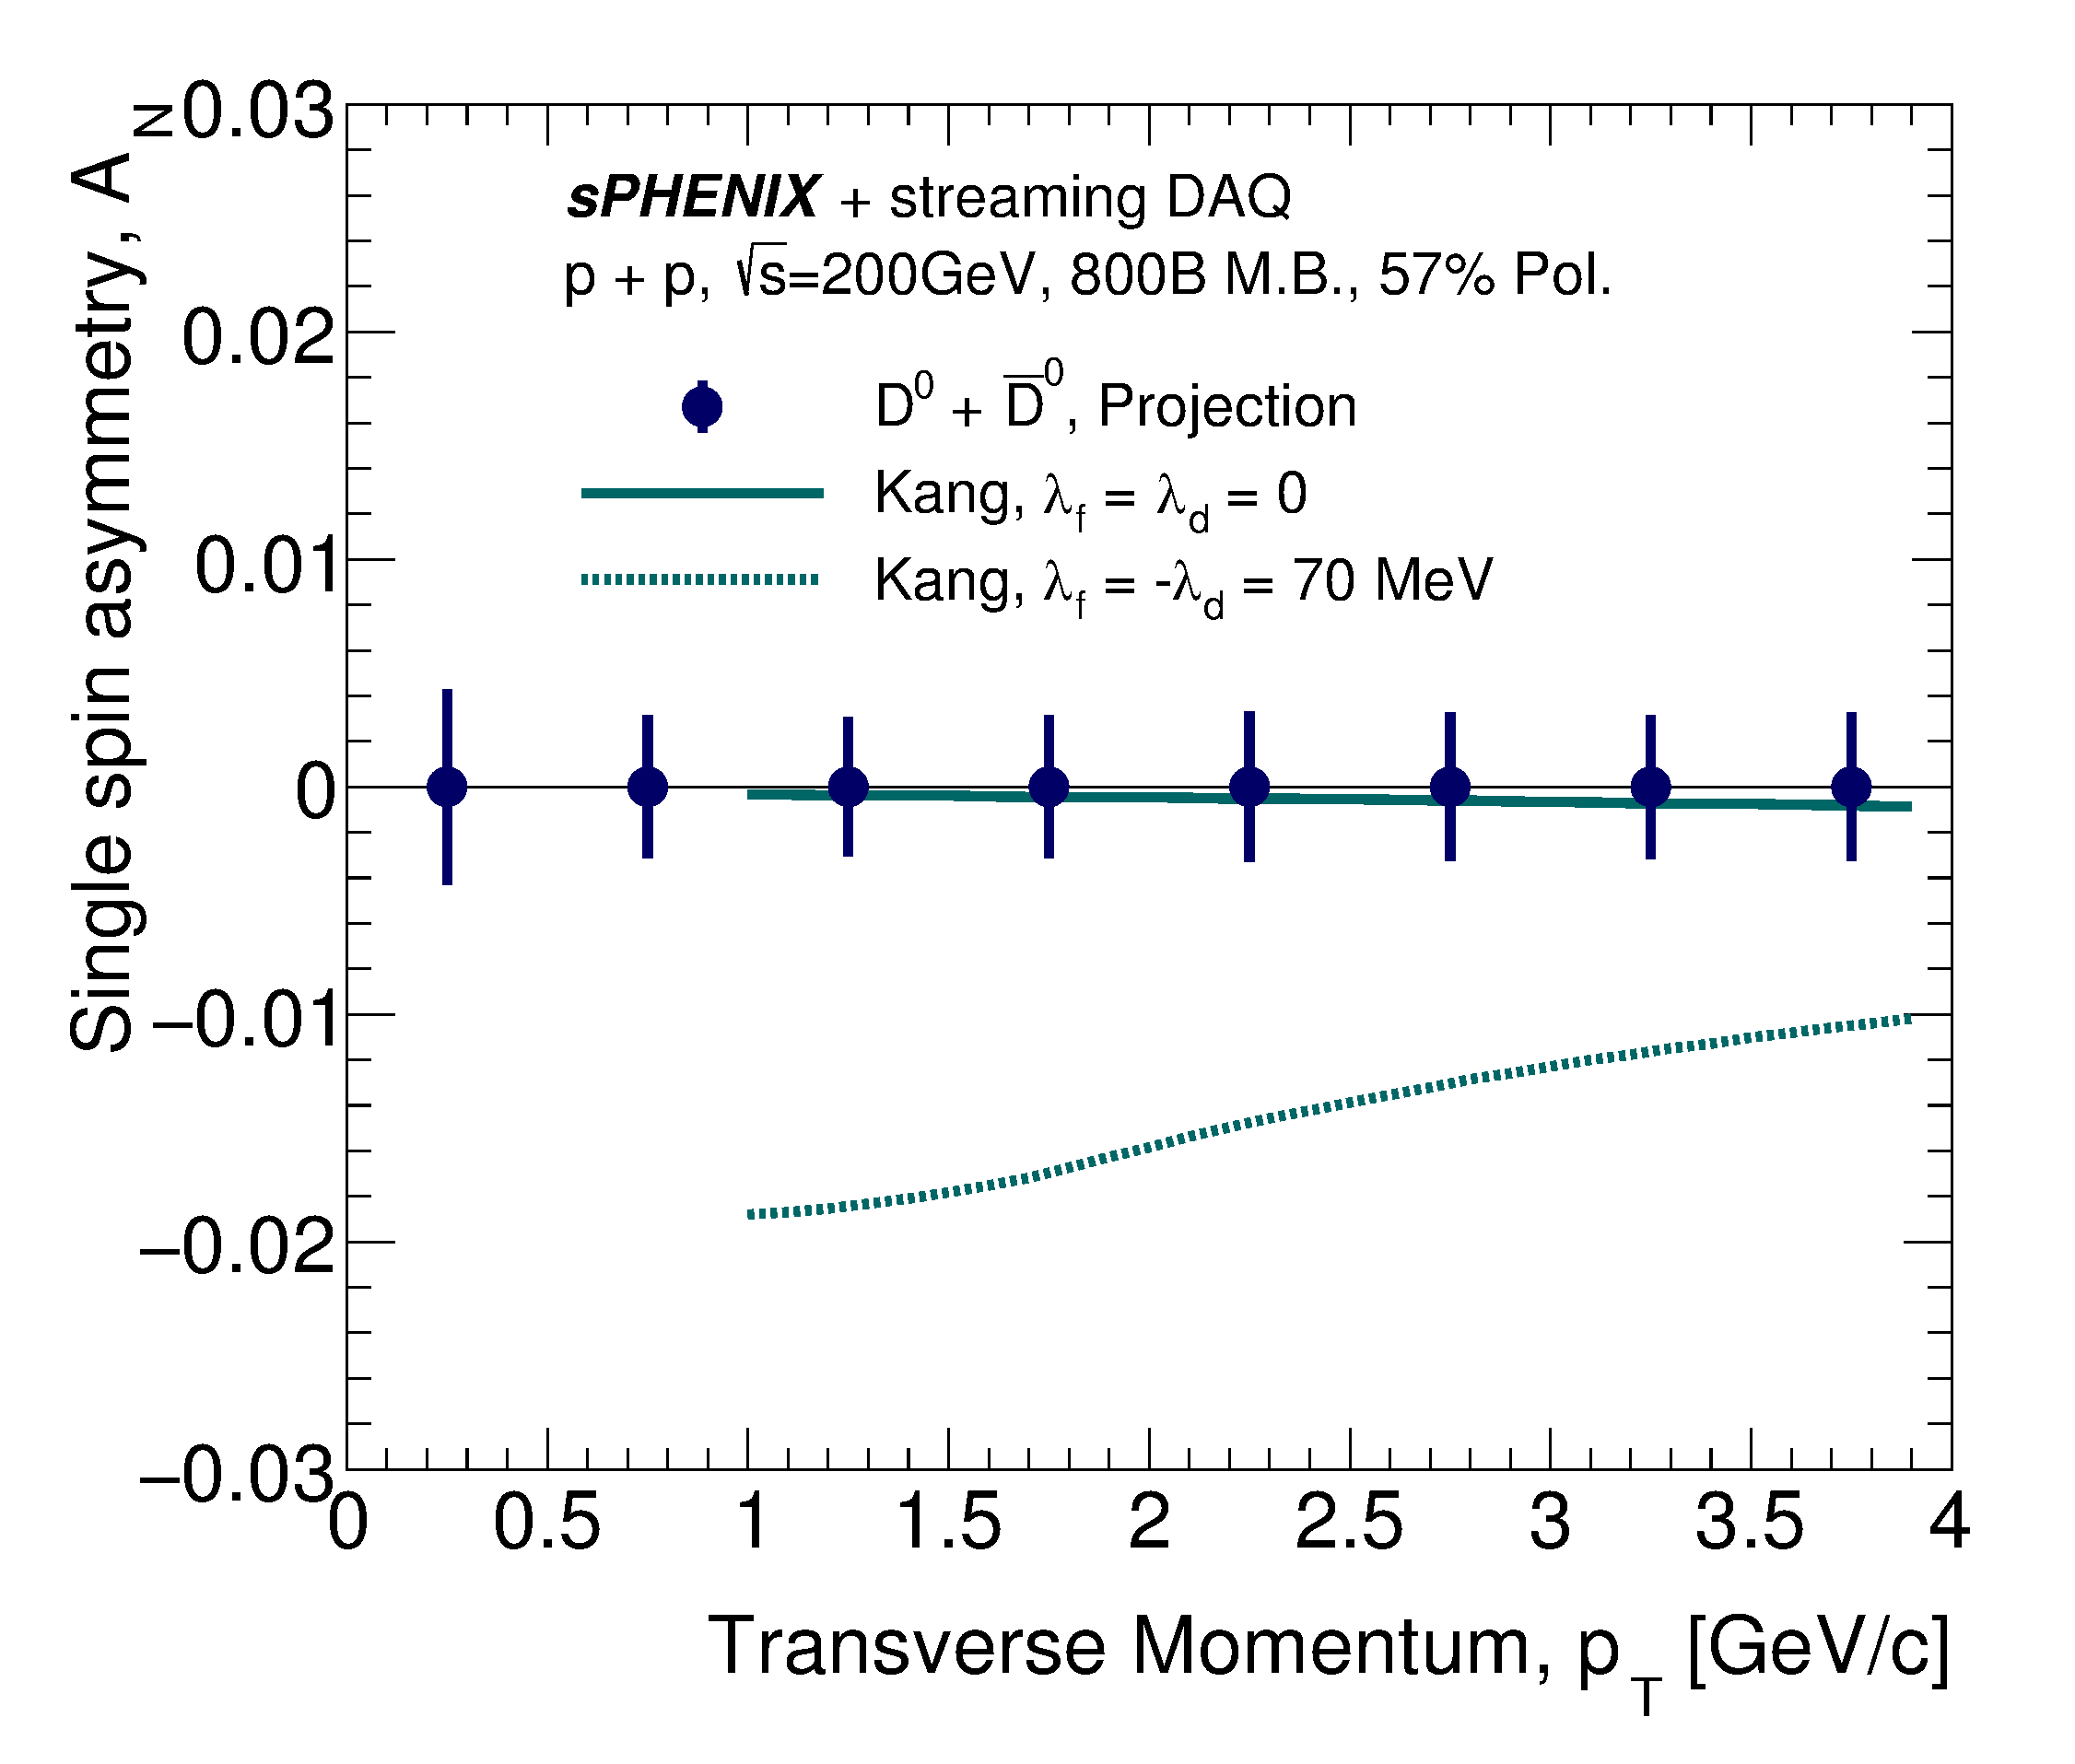
\includegraphics[width=.49\linewidth]{figs/RAA_DB_theory_root_AN_D0D0bar.pdf}
\caption{[Possible plot where  5-yr HF statistics is critical]{\textcolor{red}{[To add 2-yr comparison and upgrade luminosity to 100\% streaming. Should be very impressive improve in precision]}} Statistical projections of
  transverse spin asymmetry for the $D^0$ mesons for Year
  2+4 data taking, a dramatic improvement over the initial data discussed in Section~\ref{sec:ColdQCD}. }
\label{fig:AN-D0}
\end{center}
\end{figure}



%%%%%%%%%%%%%%%%%%%%%%%%%%%%%%%%%%%%%%%%%%%%%%%%%%%%%%%%%%%%%%%%%%%%%%%%%%%%%

\FloatBarrier

\section{O+O and Ar+Ar Physics Reach}

The RHIC program has a 100\% track record of learning new physics and gaining insights from every novel nuclear species combinations put into collision.    It is a testament to the facility and the constant improvements, including the EBIS source, that have been the lifeblood of the machine.    An opportunity to run smaller symmetric collision species of O+O and Ar+Ar is essentially guaranteed to provide key insights and resolve some key outstanding puzzles in the field.  

A major open question in the field and an associated major puzzle relates to jet quenching or the lack thereof in small systems, for example \pau at RHIC and p+Pb at the LHC.    Despite a wealth of evidence for collectivity~\cite{Nagle:2018nvi}, described by hydrodynamics in these small systems, the $p_{T}$ distribution of charged hadrons, reconstructed jets, and open heavy-flavor hadrons appears nearly unmodified, i.e. R$_{pA}$ = 1 within uncertainties.    Is there a minimum medium size or lifetime requires for jet quenching phenomena?   Does such a minimum value relate to hard struck quarks and gluons having a formation time before scattering in medium or having coherence effects?   These are fundamental questions that are needed to fully understand the physics of small systems and to bridge the divide between small and large systems.    

The associated major puzzle is that at the LHC in p+Pb collisions there is a definite azimuthal anisotropy for charged hadrons up to $p_{T} \approx 50$~GeV~\cite{Aad:2019ajj} and $D$ mesons and their decay leptons are observed to have an azimuthal anisotropy as well in p+A and even p+p collisions at the LHC.   In A+A collisions, the high-$p_T$ $v_{2}$ is interpreted as differential jet quenching, which would seem impossible in small systems if there is no indication of jet quenching in the nuclear modification factor.   sPHENIX will extend these measurements as part of the \pau running in 2024 as discussed in Section~\ref{sec:ColdQCD}.

In principle one can use peripheral \auau or Pb+Pb collisions to map out these observables and bridge the divide between large and small.   However, there are substantial event selection biases that have recently been shown to have caused R$_{AA} < 1$ in peripheral A+A collisions at RHIC and the LHC~\cite{Morsch:2017brb}.    Correcting for these biases is challenging particularly if one is teasing out modest modifications in the $p_{T}$ distribution of order 10-20\%.    One solution to this problem is to run smaller symmetric nuclear collisions.   One can use minimum bias events where there is no event selection bias, and one can also use selected high-multiplicity selected events where the bias is in the opposite direction to that in \auau and thus one can test whether one can correct out this bias.

\begin{figure}[h]
    \centering
    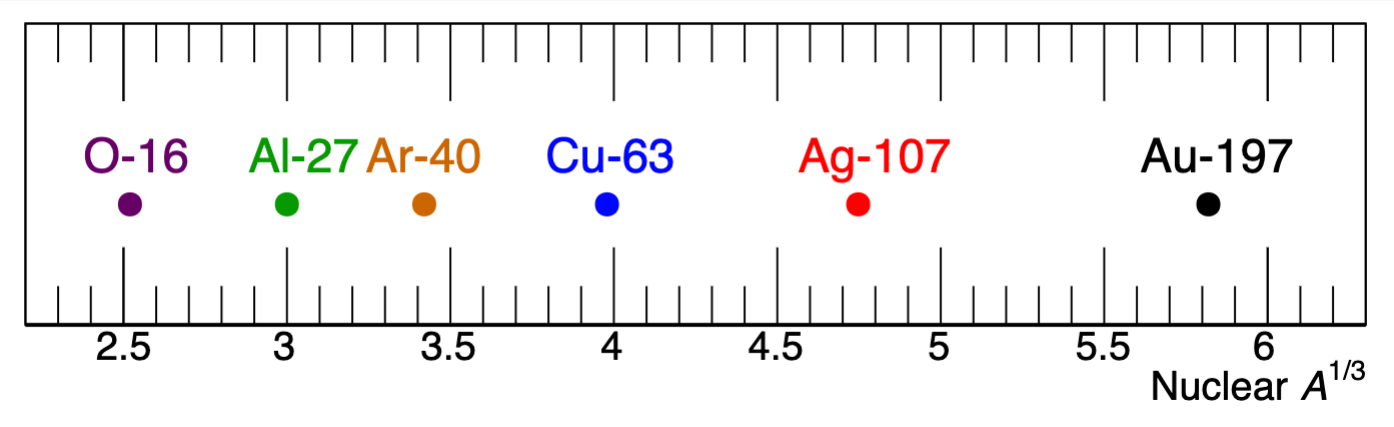
\includegraphics[width=0.85\linewidth]{figs/figure_A.png}
    \caption{Various nuclei plotted as a function of $A^{1/3}$.}
    \label{fig:figA}
\end{figure}

What is the optimum nuclear collisions species and for how many weeks should one run to collect the necessary data set?    Figure~\ref{fig:figA} shows the nuclear thickness as it scales with $A^{1/3}$ for different potential nuclei.   Monte Carlo Glauber and direct photon NLO rates are combined with C-AD luminosity projections to plot the number of direct photons 
that can be measured by sPHENIX per week of running as a function of the number of binary collisions $N_{coll}$, as shown in Figure~\ref{fig:figSmallPhoton}.

\begin{figure}[h]
    \centering
    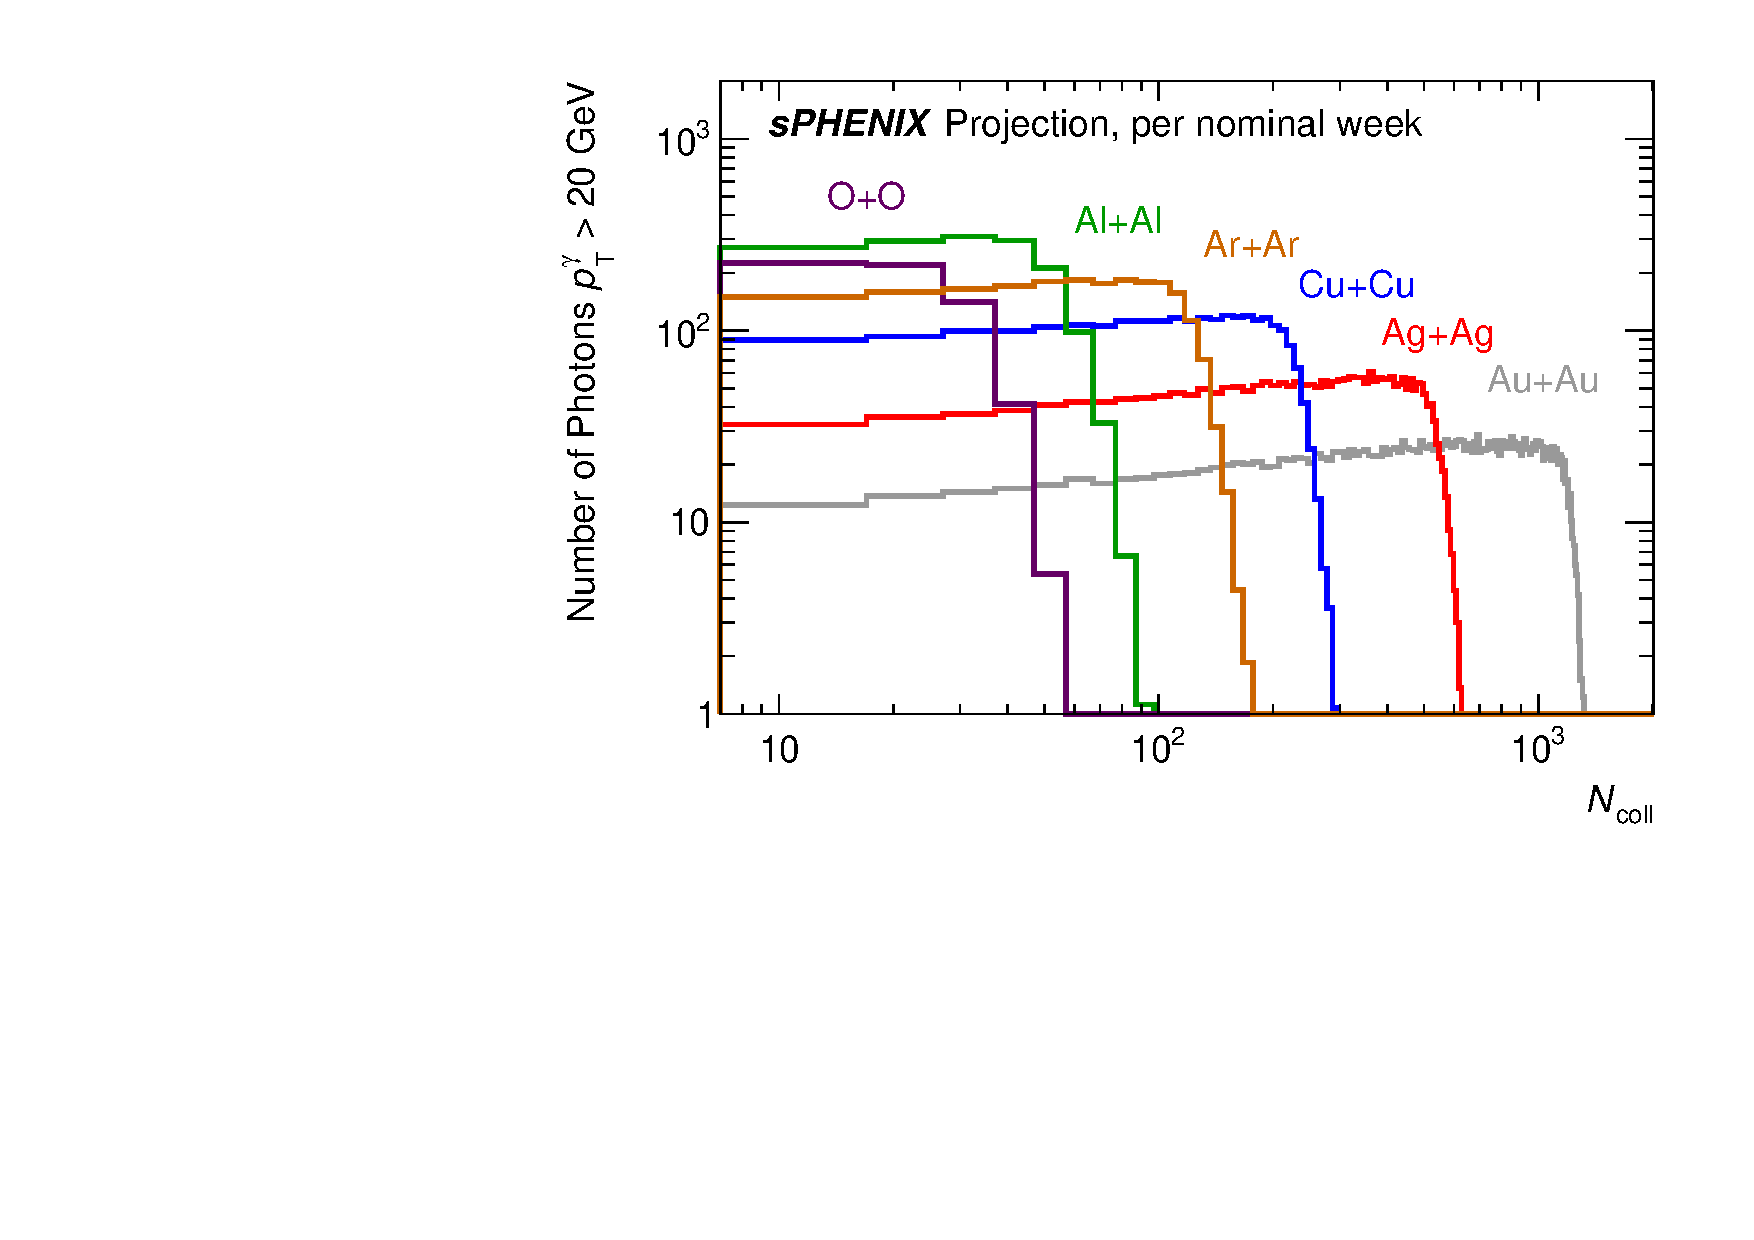
\includegraphics[width=0.48\linewidth]{figs/sPHENIX_BUP_SmallSystems_PhotonProjection}
    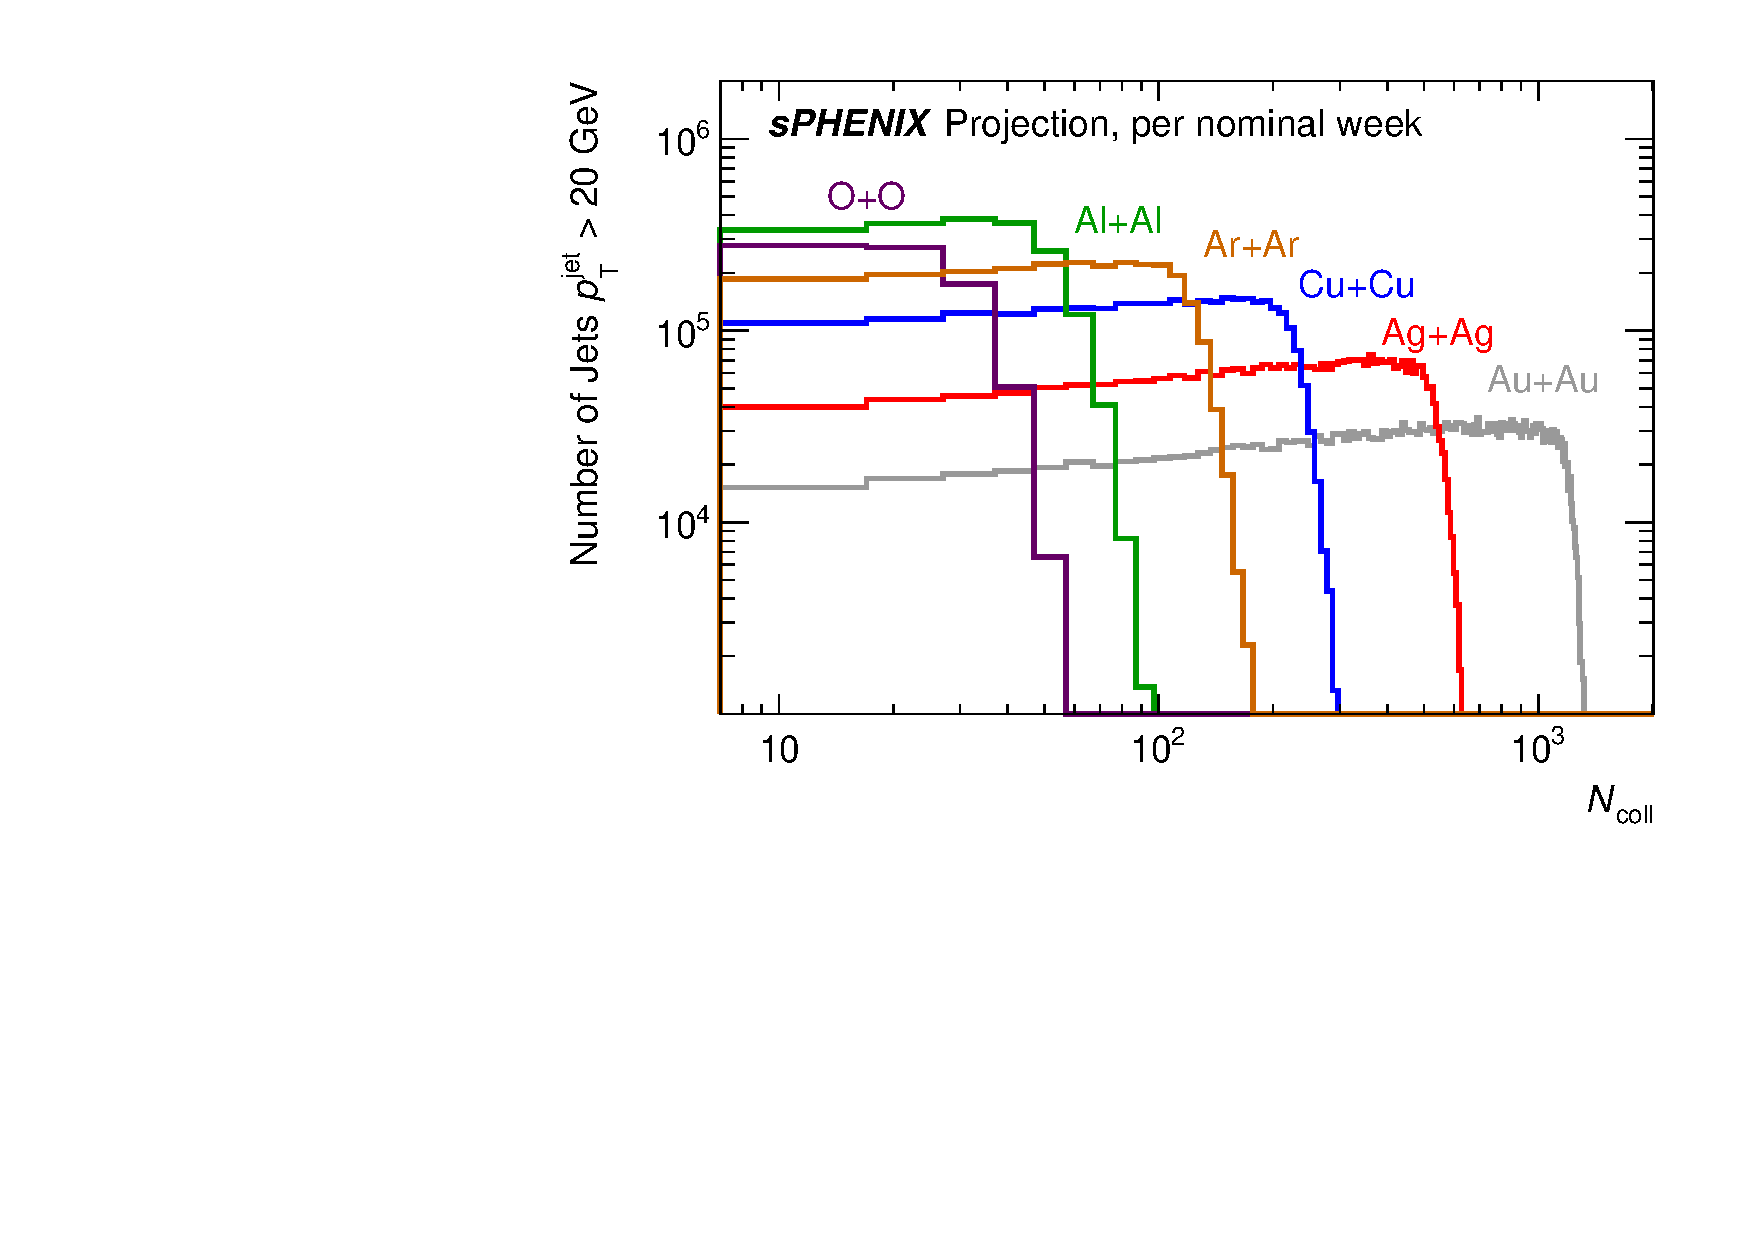
\includegraphics[width=0.48\linewidth]{figs/sPHENIX_BUP_SmallSystems_JetProjection}
    \caption{Number of direct photons (left) and jets (right) with $p_T > 20$~GeV measurable by sPHENIX per nominal week of delivered luminosity as a function of the number of binary collisions.}
    \label{fig:figSmallPhoton}
\end{figure}

An optimum balance of system size and running time is closely matched by running two-weeks of physics data taking for O+O and Ar+Ar.   Using projections from C-AD, even during this short running period, one can measure direct photons beyond 25~GeV and jets out beyond 50~GeV as shown in Figure~\ref{fig:jet_RAA_SmallSystems}.   The direct photon measurement in particular enables confirmation of minimum bias $A$-scaling of the cross section as well as any corrections to bias factors in multiplicity-selected events.    

The statistics available will also enable differential measurements of many quantities.  For example, Fig.~\ref{fig:jet_xJg_SmallSystems} shows projected $x_\mathrm{J\gamma}$ distributions for $p_\mathrm{T}^{\gamma} > 20$~GeV, for which there will be $800$ and $1\,900$ events in O+O and Ar+Ar data, respectively. The projection shows that there will significant statistics to make a compelling measurement of $gamma$-tagged energy loss in these small symmetric systems. As a note, the projection includes very low values of $x_\mathrm{J\gamma} < 0.4$ at which jet measurements may not be feasible. However, the physics effect is primarily at high $x_\mathrm{J\gamma}$ since the magnitude of energy loss is expected to be small, and one could use photon--hadron correlations to explore the very low-$p_\mathrm{T}$ physics.


\begin{figure}[h]
\centering
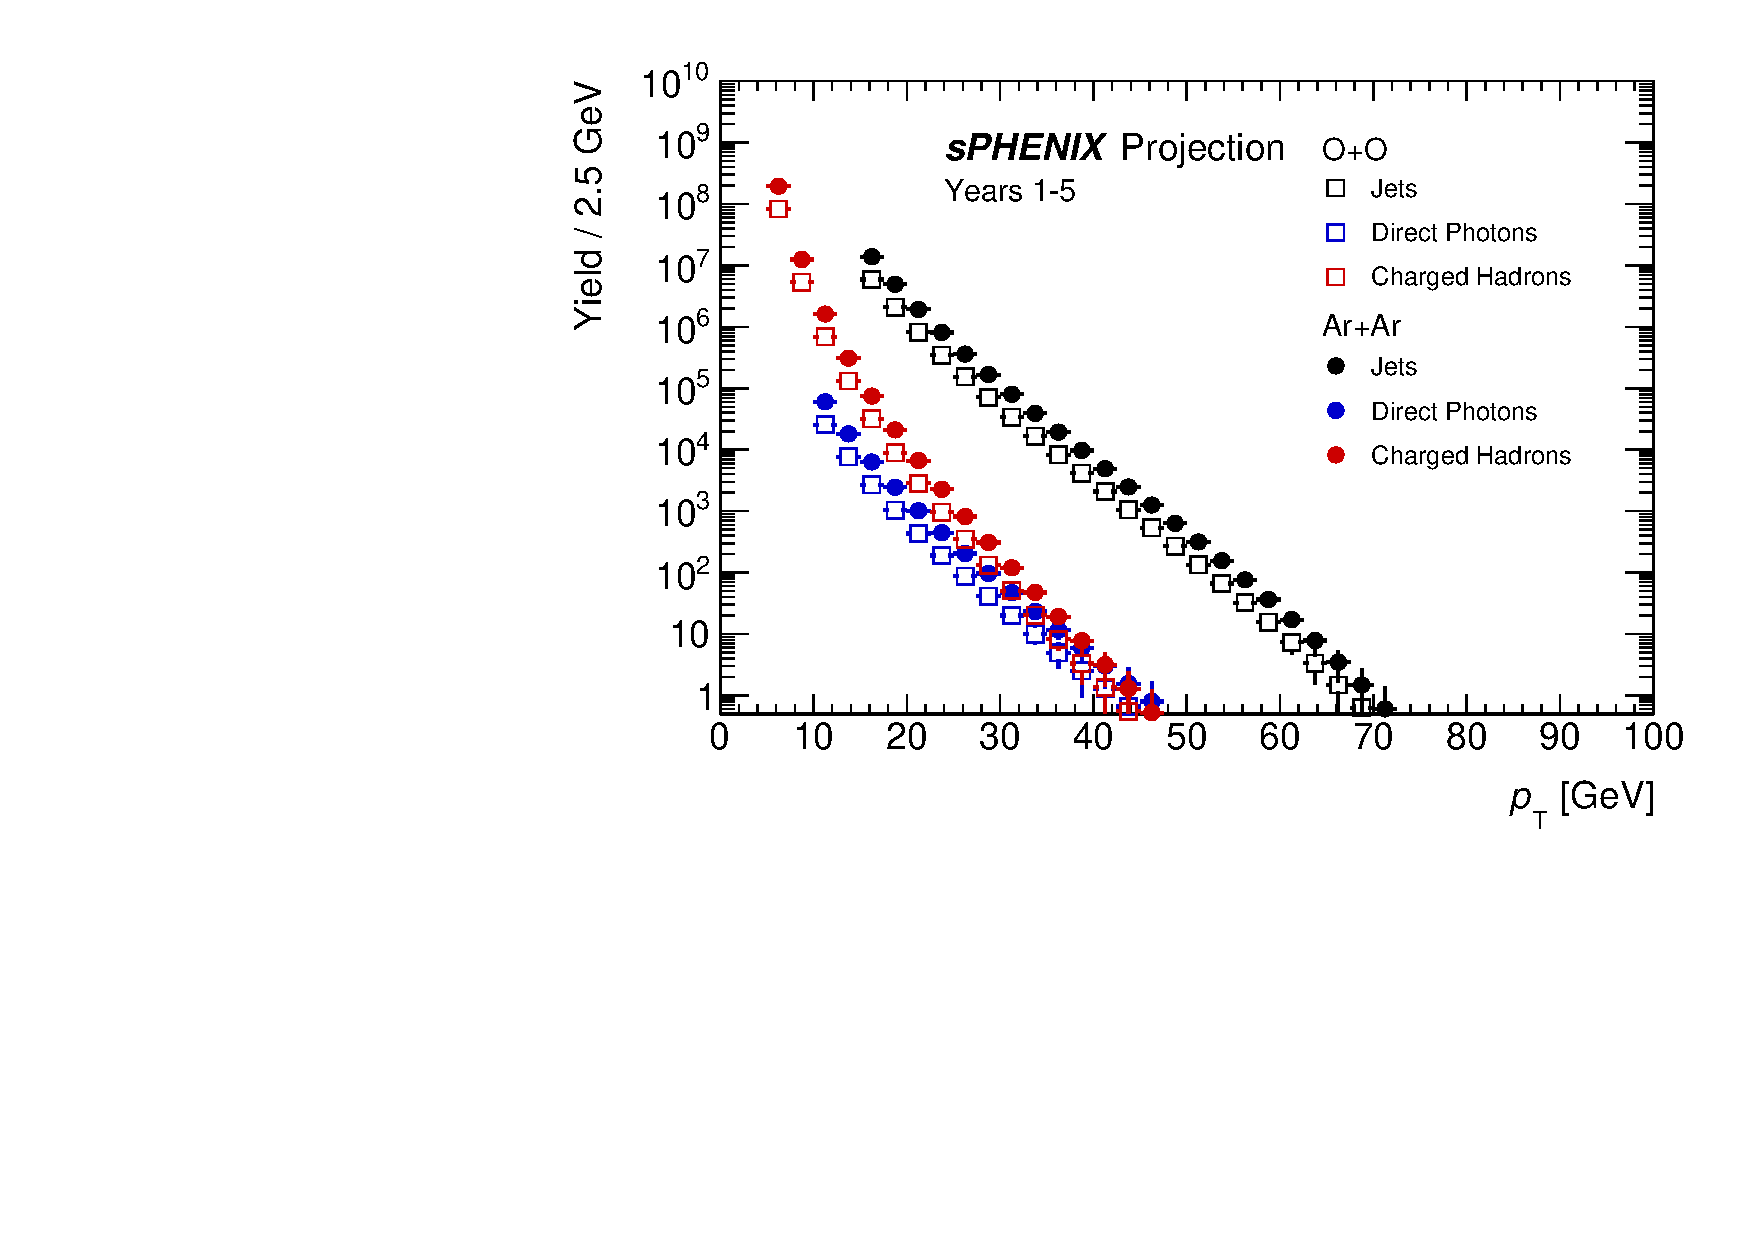
\includegraphics[width=0.48\textwidth]{figs/master_SmallSystems_yields.pdf}
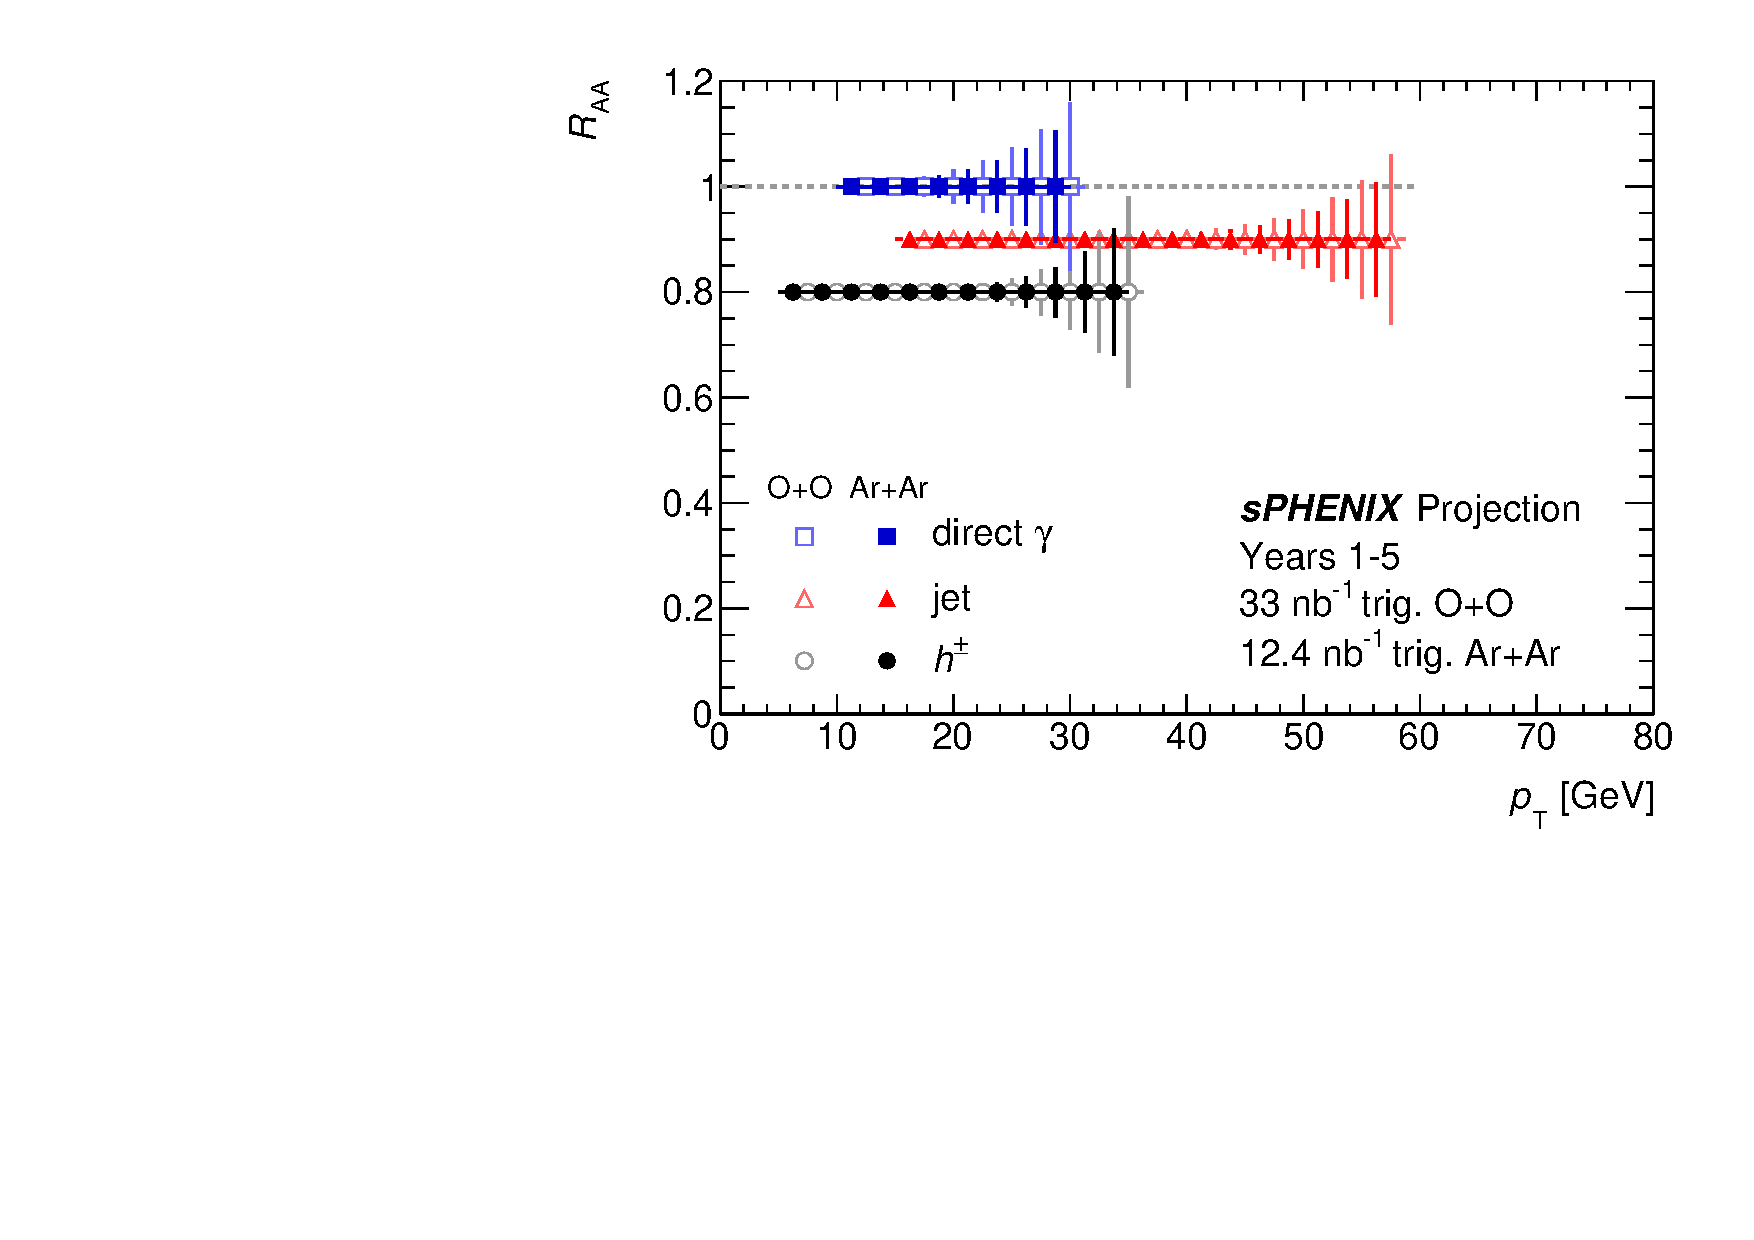
\includegraphics[width=0.48\textwidth]{figs/RAA_SmallSystems.pdf}
\caption{Projected total yields (left) and $R_\mathrm{AA}$ (right) for
  jets, photons, and charged hadrons in O+O and Ar+Ar events taken during the fourth year of sPHENIX data-taking.}
\label{fig:jet_RAA_SmallSystems}
\end{figure}

\begin{figure}[h]
\centering
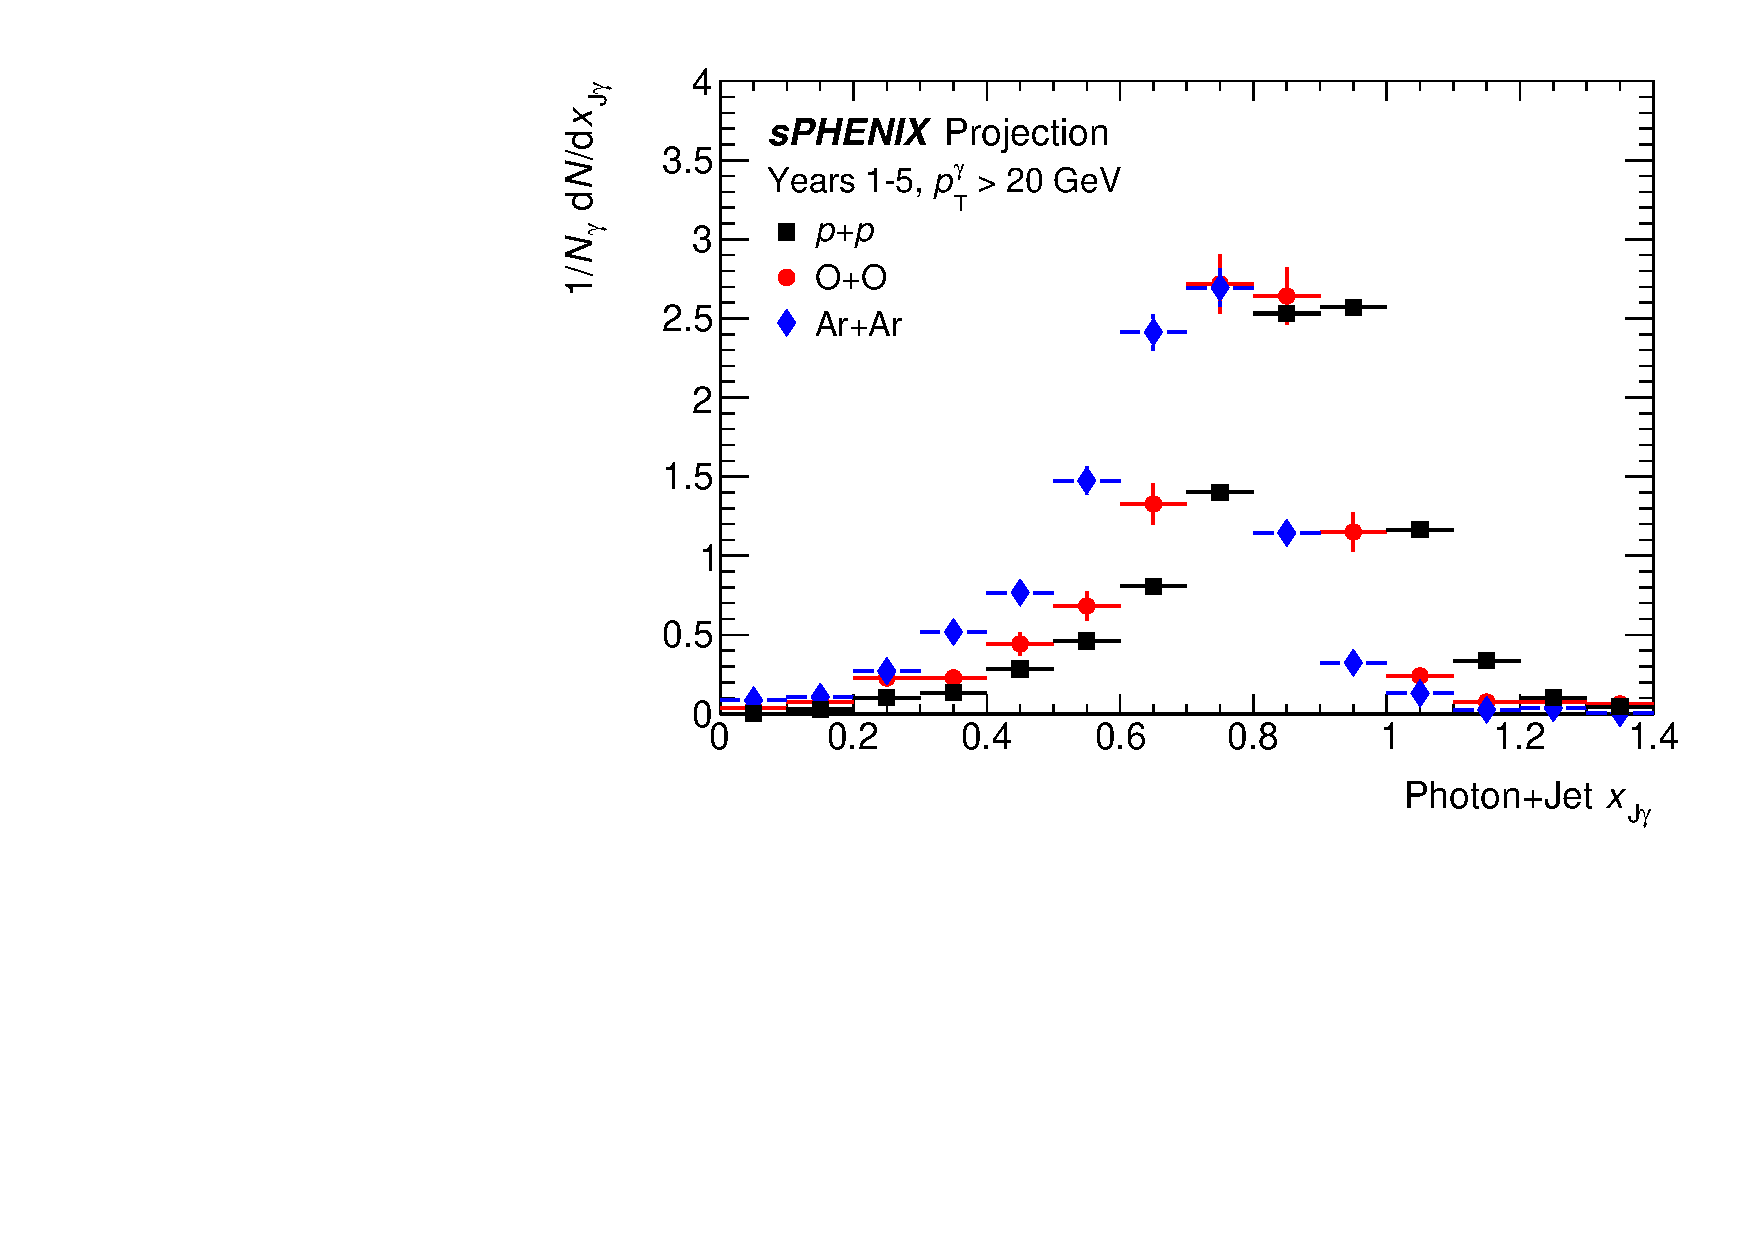
\includegraphics[width=0.48\textwidth]{figs/xJg_3}
\caption{Projected jet-to-photon $p_\mathrm{T}$ balance distributions for $p_\mathrm{T}^{\gamma} > 20$~GeV in $p$+$p$, O+O, and Ar+Ar collisions after four years of sPHENIX data-taking.}
\label{fig:jet_xJg_SmallSystems}
\end{figure}

{\textcolor{red}{COULD WE MAKE A FIGURE OF V2 FOR CHARGED HADRONS IN OO TO COMPARE WITH ATLAS PPB MEASUREMENT -- see example in Figure~\ref{fig:atlaspbhighpt}.}} {\color{red}{DVP: Yes, but after the initial circulation to the Collaboration}}

\begin{figure}
    \centering
    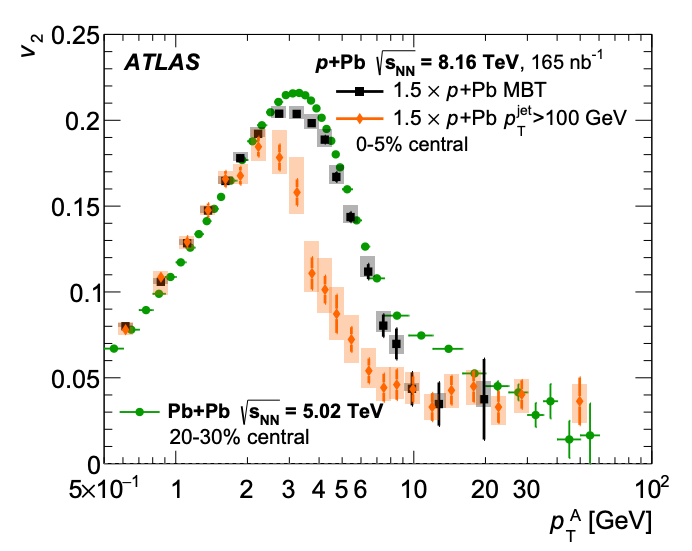
\includegraphics[width=0.47\linewidth]{figs/figure_atlas_highptv2_ppb.png}
    \caption{(left) ATLAS high-$p_{T}$ $v_{2}$ in p+Pb and Pb+Pb collisions at the LHC.
    (right) -- CAN WE GENERATE A SIMILAR FIGURE FOR O+O FOR SPHENIX? {\color{red}{DVP: Yes, but after the initial circulation to the Collaboration}}}
    \label{fig:atlaspbhighpt}
\end{figure}

Additionally, the related puzzle of heavy-flavor anisotropies in \pp and p+A but with R$_{pA} \approx 1$ can be tested in these small systems.   With the 100\% streaming readout data acquisition mode, a large minimum bias sample for $D^{0}$ and other heavy-flavor hadrons can be measured.    Measurements in O+O and Ar+Ar of heavy-flavor R$_{AA}$ and $v_{2}$ are a key part of understanding the physics in these small systems.   There are theoretical proposals that the azimuthal anisotropy in small systems for heavy-flavor hadrons and quarkonia comes from initial-state Color Glass Condensate effects.   However, this is challenged by the idea that the heavy-flavor particles are correlated with all bulk low-$p_{T}$ particles that are described by hydrodynamics.
{\textcolor{red}{GOAL IS TO GET RAA AND V2 PROJECTIONS FOR MIN.BIAS OR CENTRAL O+O AND AR+AR NEXT WEEK BEFORE WE SUBMIT THE DOCUMENT.}}

\FloatBarrier

%%%%%%%%%%%%%%%%%%%%%%%%%%%%%%%%%%%%%%%%%%%%%%%%%%%%%%%%%%%%%%%%%%%%%%%%%%%%%
\newpage
\section{Cryo-Week Details}
\label{sec:cryo20262027}

For completeness, we detail the 28 cryo-weeks of potential running in 2026 and 2027 in Table~\ref{tab:cryoplan2026} and Table~\ref{tab:cryoplan2027} respectively.

\begin{table}[hb!]
\centering
\begin{tabular}{ | c | l | }
\hline
Weeks & Designation \\ \hline
0.5  & Cool Down from 50 K to 4 K \\ \hline
2.0  & Set-up mode 1 (p$^{\uparrow}$p$^{\uparrow}$ at 200 GeV) \\ \hline
0.5  & Ramp-up mode 1 (8 h/night for experiment) \\ \hline
15.5 & Data taking mode 1 (p$^{\uparrow}$p$^{\uparrow}$ Physics) \\ \hline
2.0  & Set-up mode 2 (O+O at 200 GeV) \\ \hline
0.5  & Ramp-up mode 2 (8 h/night for experiment) \\ \hline
2.0 & Data taking mode 2 (O+O Physics) \\ \hline
2.0  & Set-up mode 3 (Ar+Ar at 200 GeV) \\ \hline
0.5  & Ramp-up mode 3 (8 h/night for experiment) \\ \hline
2.0 & Data taking mode 3 (Ar+Ar Physics) \\ \hline
0.5  & Controlled refrigeration turn-off \\ \hline \hline \hline
28.0 & Total cryo-weeks \\
\hline
\end{tabular}
\caption{Year 2026 run plan for 28 cryo-weeks with p$^{\uparrow}$p$^{\uparrow}$, O+O, and Ar+Ar 200~GeV collisions.\label{tab:cryoplan2026}}
\end{table}


\begin{table}
\centering
\begin{tabular}{ | c | l | }
\hline
Weeks & Designation \\ \hline
0.5  & Cool Down from 50 K to 4 K \\ \hline
2.0  & Set-up mode 1 (Au+Au at 200 GeV) \\ \hline
0.5  & Ramp-up mode 1 (8 h/night for experiments) \\ \hline
24.5 & Data taking mode 1 (Physics) \\ \hline
0.5  & Controlled refrigeration turn-off \\ \hline \hline \hline
28.0 & Total cryo-weeks \\
\hline
\end{tabular}
\caption{Year 2027 run plan for 28 cryo-weeks with Au+Au 200~GeV collisions.
\label{tab:cryoplan2027}}
\end{table}